% Requires in the preamble:
% \usepackage{amsmath,amssymb}
% \usepackage{tikz,pgfplots}
% \pgfplotsset{compat=1.18}

\chapter{The Fundamental Theorem of Calculus}
\label{chap:fundamental-theorem-calculus}

Chapter \ref{chap:integral-as-accumulation} built the integral as accumulated signed
change:

\[
\int_a^b f(x)\,dx.
\]

At first this integral was a number.  It accumulated from one fixed endpoint to another.

Now we let one endpoint move.

That small change turns the integral into a function.  The surprise is that this new
function has a derivative, and its derivative is the function we started with.

\[
\text{accumulate } f
\quad\Longrightarrow\quad
\text{differentiate the accumulation}
\quad\Longrightarrow\quad
f.
\]

This is the first half of the Fundamental Theorem of Calculus.

\section{Accumulation functions}
\label{sec:accumulation-functions}

A definite integral with fixed endpoints gives one accumulated amount.  But if the upper
endpoint moves, the accumulated amount changes.  That changing amount is a function.

This is the same idea as an odometer.  At each time, the odometer reading is the
accumulated velocity up to that time.  If we know the velocity graph, then the odometer
reading is an area-with-sign whose right endpoint moves.

\subsection{Area with a moving endpoint}
\label{subsec:area-moving-endpoint}

Start with a simple height function,

\[
f(t)=2+t,
\qquad t\ge 0.
\]

Let \(A(x)\) be the area under \(f\) from \(0\) to \(x\):

\[
A(x)=\int_0^x (2+t)\,dt,
\qquad x\ge 0.
\]

Because \(f(t)=2+t\) is a line, we can compute this area by geometry.  The region is a
rectangle of height \(2\) and width \(x\), plus a right triangle of base \(x\) and height
\(x\).

So

\[
A(x)=2x+\frac12 x^2.
\]

\begin{figure}[h]
\centering
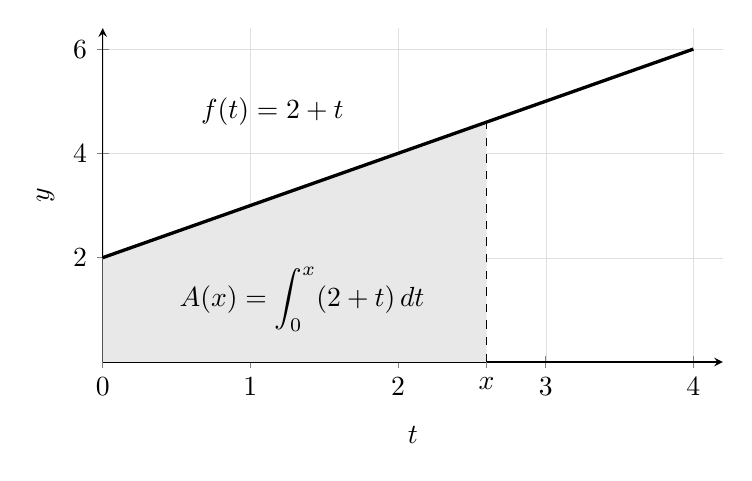
\begin{tikzpicture}
\begin{axis}[
    width=0.78\textwidth,
    height=0.48\textwidth,
    xmin=0, xmax=4.2,
    ymin=0, ymax=6.4,
    axis lines=left,
    xlabel={\(t\)},
    ylabel={\(y\)},
    xtick={0,1,2,3,4},
    ytick={2,4,6},
    extra x ticks={2.6},
    extra x tick labels={\(x\)},
    extra x tick style={grid=none},
    grid=both,
    grid style={line width=.1pt, draw=gray!25},
]
\addplot[domain=0:2.6, samples=2, fill=gray!18, draw=none] {2+x} \closedcycle;
\addplot[very thick, domain=0:4, samples=2] {2+x};
\draw[dashed] (axis cs:2.6,0) -- (axis cs:2.6,4.6);
\node[anchor=west] at (axis cs:0.6,4.8) {\(f(t)=2+t\)};
\node at (axis cs:1.35,1.2) {\(A(x)=\displaystyle\int_0^x (2+t)\,dt\)};
\end{axis}
\end{tikzpicture}
\caption{As the right endpoint \(x\) moves, the accumulated area \(A(x)\) changes.}
\label{fig:area-moving-endpoint-line}
\end{figure}

Now ask how fast this accumulated area changes as \(x\) changes.

Since

\[
A(x)=2x+\frac12x^2,
\]

we have

\[
A'(x)=2+x.
\]

But

\[
2+x=f(x).
\]

So in this example,

\[
\boxed{A'(x)=f(x).}
\]

The slope of the accumulated area function is the current height of the graph.

This is not an accident.  It is the central pattern.

\subsection{\texorpdfstring{\(A(x)=\int_a^x f(t)\,dt\)}{A(x)=int_a^x f(t) dt}}
\label{subsec:accumulation-function-definition}

Let \(f\) be integrable on an interval containing \(a\).  Fix the starting point \(a\).  Define

\[
\boxed{
A(x)=\int_a^x f(t)\,dt.
}
\]

This \(A\) is called an \emph{accumulation function}.

The variable \(t\) is a placeholder inside the integral.  We use \(t\) instead of \(x\)
because \(x\) is already being used for the moving endpoint.  The expressions

\[
\int_a^x f(t)\,dt
\]

and

\[
\int_a^x f(u)\,du
\]

mean the same thing.  The letter inside the integral is temporary.  The endpoint \(x\)
is not temporary; it is the input to the new function \(A\).

\paragraph{Example.}
If

\[
f(t)=t^2
\]

and

\[
A(x)=\int_1^x t^2\,dt,
\]

then \(A(3)\) is the accumulated area under \(t^2\) from \(1\) to \(3\):

\[
A(3)=\int_1^3 t^2\,dt.
\]

The number \(A(2)\) is

\[
A(2)=\int_1^2 t^2\,dt.
\]

The function \(A(x)\) stores all such accumulated areas at once.

\paragraph{Orientation still matters.}
If \(x>a\), then

\[
A(x)=\int_a^x f(t)\,dt
\]

accumulates in the usual left-to-right direction.

If \(x<a\), then

\[
A(x)=\int_a^x f(t)\,dt
=
-\int_x^a f(t)\,dt.
\]

So even when \(f(t)\ge0\), the value of \(A(x)\) can be negative for \(x<a\).  The sign
comes from the direction of accumulation.

\[
\boxed{
\text{The endpoint \(x\) moves.  The direction from \(a\) to \(x\) is part of the meaning.}
}
\]

\subsection{Estimating the change in an accumulation function}
\label{subsec:estimating-change-accumulation-function}

The derivative of \(A\) begins with a difference quotient:

\[
\frac{A(x+h)-A(x)}{h}.
\]

Because \(A\) is an integral, the numerator is a difference of accumulated amounts:

\[
A(x+h)-A(x)
=
\int_a^{x+h} f(t)\,dt-\int_a^x f(t)\,dt.
\]

By additivity of the integral over intervals,

\[
\int_a^{x+h} f(t)\,dt
=
\int_a^x f(t)\,dt+\int_x^{x+h} f(t)\,dt.
\]

Therefore

\[
\boxed{
A(x+h)-A(x)=\int_x^{x+h} f(t)\,dt.
}
\]

This identity is the key.  The change in accumulated area is the small new strip from
\(x\) to \(x+h\).

\begin{figure}[h]
\centering
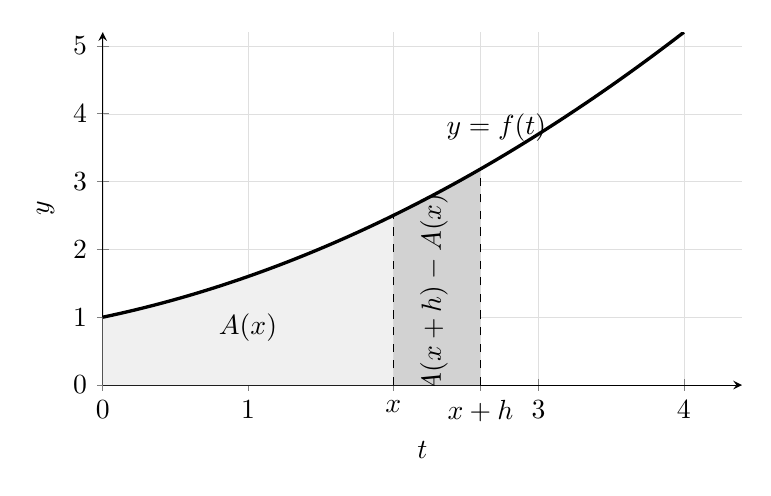
\begin{tikzpicture}
\begin{axis}[
    width=0.80\textwidth,
    height=0.50\textwidth,
    xmin=0, xmax=4.4,
    ymin=0, ymax=5.2,
    axis lines=left,
    xlabel={\(t\)},
    ylabel={\(y\)},
    xtick={0,1,2,2.6,3,4},
    xticklabels={\(0\),\(1\),\(x\),\(x+h\),\(3\),\(4\)},
    ytick={0,1,2,3,4,5},
    grid=both,
    grid style={line width=.1pt, draw=gray!25},
]
% accumulated area up to x=2
\addplot[domain=0:2, samples=100, fill=gray!12, draw=none] {1+0.45*x+0.15*x^2} \closedcycle;
% new strip from x to x+h
\addplot[domain=2:2.6, samples=100, fill=gray!35, draw=none] {1+0.45*x+0.15*x^2} \closedcycle;
% curve
\addplot[very thick, domain=0:4, samples=150] {1+0.45*x+0.15*x^2};
\draw[dashed] (axis cs:2,0) -- (axis cs:2,2.5);
\draw[dashed] (axis cs:2.6,0) -- (axis cs:2.6,3.184);
\node[anchor=center] at (axis cs:1.0,0.85) {\(A(x)\)};
\node[rotate=90, anchor=center] at (axis cs:2.28,1.35) {\(A(x+h)-A(x)\)};
\node[anchor=west] at (axis cs:2.3,3.8) {\(y=f(t)\)};
\end{axis}
\end{tikzpicture}
\caption{The change in an accumulation function is the thin strip from \(x\) to \(x+h\).}
\label{fig:accumulation-change-strip}
\end{figure}

If \(h>0\), the strip has width \(h\).  If \(h<0\), the strip is traversed in the opposite
direction, and the same formula still works.

For small \(h\), and for a continuous \(f\), the graph does not change much between
\(x\) and \(x+h\).  The strip is approximately a rectangle with height \(f(x)\) and width
\(h\).  Therefore

\[
A(x+h)-A(x)
=
\int_x^{x+h} f(t)\,dt
\approx
f(x)h.
\]

Divide by \(h\):

\[
\frac{A(x+h)-A(x)}{h}
\approx
f(x).
\]

As \(h\to0\), this approximation should become exact.

\subsection{The slope of accumulated area}
\label{subsec:slope-accumulated-area}

For \(h>0\), the difference quotient becomes

\[
\frac{A(x+h)-A(x)}{h}
=
\frac1h\int_x^{x+h} f(t)\,dt.
\]

The right side has a direct meaning:

\[
\boxed{
\frac1h\int_x^{x+h} f(t)\,dt
=
\text{average value of \(f\) on }[x,x+h].
}
\]

So the slope of the accumulation function over \([x,x+h]\) is the average height of the
original function over that same interval.

As the interval shrinks, the average height should approach the current height, provided
there is no jump at \(x\).

\[
\text{average height near \(x\)}
\longrightarrow
\text{height at \(x\)}.
\]

That is why we expect

\[
A'(x)=f(x).
\]

\paragraph{Example: the line again.}
Let

\[
A(x)=\int_0^x (2+t)\,dt.
\]

From geometry,

\[
A(x)=2x+\frac12x^2.
\]

Then

\[
A(x+h)-A(x)
=
\left(2(x+h)+\frac12(x+h)^2\right)
-
\left(2x+\frac12x^2\right).
\]

Simplify:

\[
A(x+h)-A(x)
=
2h+xh+\frac12h^2.
\]

So

\[
\frac{A(x+h)-A(x)}{h}
=
2+x+\frac12h.
\]

Let \(h\to0\):

\[
A'(x)=2+x.
\]

But the original height function was

\[
f(x)=2+x.
\]

Again,

\[
A'(x)=f(x).
\]

The example has given the pattern.  The next section turns the pattern into a theorem.

\section{Fundamental Theorem, Part I}
\label{sec:fundamental-theorem-part-i}

The previous section discovered the idea:

\[
\frac{A(x+h)-A(x)}{h}
=
\text{average height of \(f\) near \(x\)}.
\]

If \(f\) is continuous, then nearby heights of \(f\) are close to \(f(x)\).  So the average
height over a tiny interval should approach \(f(x)\).

This is the first part of the Fundamental Theorem of Calculus.

\subsection{The derivative of an accumulation function}
\label{subsec:derivative-accumulation-function}

\begin{quote}
\textbf{Fundamental Theorem of Calculus, Part I.}
Let \(f\) be continuous on an interval \(I\), and fix a number \(a\in I\).  Define

\[
A(x)=\int_a^x f(t)\,dt.
\]

Then \(A\) is differentiable at every interior point \(x\) of \(I\), and

\[
\boxed{
A'(x)=f(x).
}
\]
\end{quote}

In words:

\[
\boxed{
\text{The derivative of accumulated \(f\) is \(f\) itself.}
}
\]

This theorem is the first precise statement that differentiation and integration undo each
other.

It says:

\[
\text{integrate first, then differentiate}
\quad\Longrightarrow\quad
\text{return to the original function.}
\]

\subsection{Continuity as the needed hypothesis}
\label{subsec:continuity-needed-ftc1}

The word \emph{continuous} is not decoration.  It prevents a hidden jump inside the
thin strip.

Consider the step function

\[
f(t)=
\begin{cases}
0, & t<0,\\
1, & t\ge 0.
\end{cases}
\]

Define

\[
A(x)=\int_0^x f(t)\,dt.
\]

If \(x<0\), then \(f(t)=0\) on the interval from \(x\) to \(0\), except possibly at the
endpoint \(0\), which does not affect the integral.  Therefore

\[
A(x)=0.
\]

If \(x>0\), then \(f(t)=1\) on \([0,x]\), so

\[
A(x)=x.
\]

Also,

\[
A(0)=0.
\]

Thus

\[
A(x)=
\begin{cases}
0, & x\le 0,\\
x, & x>0.
\end{cases}
\]

The graph of \(A\) has a corner at \(0\).  Its left-hand slope is \(0\), while its right-hand
slope is \(1\).  So \(A'(0)\) does not exist.

\begin{figure}[h]
\centering
\begin{minipage}{0.47\textwidth}
\centering
\begin{tikzpicture}
\begin{axis}[
    width=\textwidth,
    height=0.72\textwidth,
    xmin=-2, xmax=2,
    ymin=-0.25, ymax=1.4,
    axis lines=middle,
    xlabel={\(t\)},
    ylabel={\(f(t)\)},
    xtick={-1,0,1},
    ytick={0,1},
    grid=both,
    grid style={line width=.1pt, draw=gray!25},
    title={jump in \(f\)}
]
\addplot[very thick, domain=-2:-0.02, samples=2] {0};
\addplot[very thick, domain=0.02:2, samples=2] {1};
\addplot[only marks, mark=*, mark size=2pt] coordinates {(0,1)};
\addplot[only marks, mark=o, mark size=2.5pt, thick] coordinates {(0,0)};
\end{axis}
\end{tikzpicture}
\end{minipage}
\hfill
\begin{minipage}{0.47\textwidth}
\centering
\begin{tikzpicture}
\begin{axis}[
    width=\textwidth,
    height=0.72\textwidth,
    xmin=-2, xmax=2,
    ymin=-0.25, ymax=2.2,
    axis lines=middle,
    xlabel={\(x\)},
    ylabel={\(A(x)\)},
    xtick={-1,0,1,2},
    ytick={0,1,2},
    grid=both,
    grid style={line width=.1pt, draw=gray!25},
    title={corner in \(A\)}
]
\addplot[very thick, domain=-2:0, samples=2] {0};
\addplot[very thick, domain=0:2, samples=2] {x};
\addplot[only marks, mark=*] coordinates {(0,0)};
\node[anchor=center] at (axis cs:0.65,1.35) {\(A(x)=x\)};
\node[anchor=east] at (axis cs:-0.1,0.2) {\(A(x)=0\)};
\end{axis}
\end{tikzpicture}
\end{minipage}
\caption{A jump in \(f\) can produce a corner in the accumulation function \(A\).}
\label{fig:ftc1-step-counterexample}
\end{figure}

The problem is exactly what the theorem avoids.  Near \(0\), the function \(f\) has no
single nearby height.  From the left it is \(0\).  From the right it is \(1\).  The average
height over a shrinking interval depends on the side from which we approach.

Continuity gives one nearby height.  That is why it appears in the theorem.

\begin{quote}
\textbf{Moral.}
The conclusion

\[
\frac{d}{dx}\int_a^x f(t)\,dt=f(x)
\]

is guaranteed when \(f\) is continuous.  At a jump, the accumulation function may have
a corner.
\end{quote}

Continuity is a safe hypothesis, not the weakest possible one.  But it is the right
hypothesis for a first version of the theorem because it matches the geometry exactly:
short intervals around \(x\) have heights close to \(f(x)\).

\subsection{Geometric proof idea}
\label{subsec:ftc1-geometric-proof-idea}

The proof is almost contained in one picture.

Let

\[
A(x)=\int_a^x f(t)\,dt.
\]

Then

\[
A(x+h)-A(x)=\int_x^{x+h} f(t)\,dt.
\]

This is the signed area of a thin strip.

If \(f\) is continuous at \(x\), then for small \(h\), all the heights \(f(t)\) in that strip are
close to \(f(x)\).  The strip is squeezed between two rectangles whose heights are close
to \(f(x)\).

\begin{figure}[h]
\centering
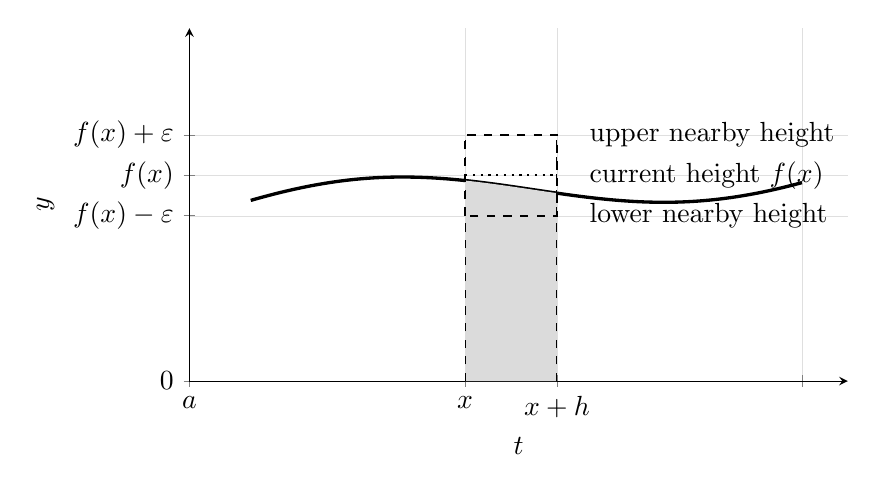
\begin{tikzpicture}
\begin{axis}[
    width=0.82\textwidth,
    height=0.50\textwidth,
    xmin=0, xmax=4.3,
    ymin=0, ymax=4.8,
    axis lines=left,
    xlabel={\(t\)},
    ylabel={\(y\)},
    xtick={0,1.8,2.4,4},
    xticklabels={\(a\),\(x\),\(x+h\),{}},
    ytick={0,2.25,2.8,3.35},
    yticklabels={\(0\),\(f(x)-\varepsilon\),\(f(x)\),\(f(x)+\varepsilon\)},
    grid=both,
    grid style={line width=.1pt, draw=gray!25},
]
% curve
\addplot[very thick, domain=0.4:4.0, samples=150] {2.2 + 0.35*sin(deg(1.4*x)) + 0.18*x};
% strip under curve
\addplot[domain=1.8:2.4, samples=80, fill=gray!28, draw=none] {2.2 + 0.35*sin(deg(1.4*x)) + 0.18*x} \closedcycle;
% bounding rectangles over strip
\draw[thick, dashed] (axis cs:1.8,2.25) rectangle (axis cs:2.4,3.35);
\draw[dotted, thick] (axis cs:1.8,2.8) -- (axis cs:2.4,2.8);
\draw[dashed] (axis cs:1.8,0) -- (axis cs:1.8,3.35);
\draw[dashed] (axis cs:2.4,0) -- (axis cs:2.4,3.35);
\node[anchor=west] at (axis cs:2.55,3.35) {upper nearby height};
\node[anchor=west] at (axis cs:2.55,2.25) {lower nearby height};
\node[anchor=west] at (axis cs:2.55,2.8) {current height \(f(x)\)};
\end{axis}
\end{tikzpicture}
\caption{Continuity squeezes the average height of a thin strip toward \(f(x)\).}
\label{fig:ftc1-squeeze-strip}
\end{figure}

After dividing by the width \(h\), the difference quotient is squeezed between heights
close to \(f(x)\).  Therefore the difference quotient approaches \(f(x)\).

\subsection{Proof of Part I}
\label{subsec:proof-ftc1}

\paragraph{Proof.}
Fix an interior point \(x\in I\).  We want to show

\[
A'(x)=f(x),
\]

which means

\[
\lim_{h\to0}\frac{A(x+h)-A(x)}{h}=f(x).
\]

First use additivity of the integral:

\[
A(x+h)-A(x)=\int_x^{x+h} f(t)\,dt.
\]

Therefore

\[
\frac{A(x+h)-A(x)}{h}
=
\frac1h\int_x^{x+h} f(t)\,dt.
\]

Subtract \(f(x)\).  Since

\[
f(x)=\frac1h\int_x^{x+h} f(x)\,dt,
\]

we get

\[
\frac{A(x+h)-A(x)}{h}-f(x)
=
\frac1h\int_x^{x+h}\bigl(f(t)-f(x)\bigr)\,dt.
\]

Now use continuity.  Let \(\varepsilon>0\).  Since \(f\) is continuous at \(x\), there is a
\(\delta>0\) such that

\[
|t-x|<\delta
\quad\Longrightarrow\quad
|f(t)-f(x)|<\varepsilon.
\]

If \(0<|h|<\delta\), then every \(t\) between \(x\) and \(x+h\) satisfies

\[
|t-x|<\delta.
\]

Thus

\[
|f(t)-f(x)|<\varepsilon
\]

throughout the small interval.

Using the order property of the integral,

\[
\left|
\int_x^{x+h}\bigl(f(t)-f(x)\bigr)\,dt
\right|
\le
\varepsilon |h|.
\]

Therefore

\[
\left|
\frac{A(x+h)-A(x)}{h}-f(x)
\right|
\le
\frac{\varepsilon |h|}{|h|}
=
\varepsilon.
\]

Since this can be done for every \(\varepsilon>0\),

\[
\lim_{h\to0}
\frac{A(x+h)-A(x)}{h}
=
f(x).
\]

So

\[
\boxed{A'(x)=f(x).}
\]

This proves the theorem. \(\square\)

\subsection{Examples with variable upper limits}
\label{subsec:examples-variable-upper-limits}

The theorem gives derivatives of functions that may be difficult, or even impossible, to
write using elementary formulas.

\paragraph{Example: an accumulation with no simple antiderivative.}
Let

\[
G(x)=\int_2^x \sqrt{1+t^4}\,dt.
\]

The integrand

\[
\sqrt{1+t^4}
\]

is continuous for all real \(t\).  Therefore the Fundamental Theorem, Part I, gives

\[
\boxed{
G'(x)=\sqrt{1+x^4}.
}
\]

We did not have to evaluate the integral.  We only had to recognize it as accumulated
area with moving endpoint \(x\).

\paragraph{Example: a moving endpoint inside another function.}
Let

\[
H(x)=\int_0^{x^2} \cos(t^3)\,dt.
\]

The upper endpoint is not \(x\).  It is \(x^2\).  Define

\[
A(u)=\int_0^u \cos(t^3)\,dt.
\]

Then

\[
H(x)=A(x^2).
\]

By the Fundamental Theorem,

\[
A'(u)=\cos(u^3).
\]

Now use the chain rule:

\[
H'(x)=A'(x^2)\cdot 2x.
\]

Since

\[
A'(x^2)=\cos\bigl((x^2)^3\bigr)=\cos(x^6),
\]

we get

\[
\boxed{
H'(x)=2x\cos(x^6).
}
\]

The chain rule is still doing its old job.  The outside function is an accumulation
function.

\paragraph{Example: a moving lower limit.}
Let

\[
K(x)=\int_x^4 e^{-t^2}\,dt.
\]

The variable \(x\) is in the lower limit.  Rewrite the integral by reversing the direction:

\[
K(x)=-\int_4^x e^{-t^2}\,dt.
\]

Now the upper endpoint is \(x\).  The Fundamental Theorem gives

\[
\frac{d}{dx}\int_4^x e^{-t^2}\,dt=e^{-x^2}.
\]

Therefore

\[
\boxed{
K'(x)=-e^{-x^2}.
}
\]

The minus sign comes from orientation.  Increasing the lower limit removes area from
the interval of accumulation.

\paragraph{Example: two moving limits.}
Let

\[
P(x)=\int_{\sin x}^{x^2} (1+t^2)\,dt.
\]

Split the integral at \(0\):

\[
P(x)
=
\int_0^{x^2}(1+t^2)\,dt
-
\int_0^{\sin x}(1+t^2)\,dt.
\]

For the first term, define

\[
A(u)=\int_0^u (1+t^2)\,dt.
\]

Then

\[
A'(u)=1+u^2,
\]

so

\[
\frac{d}{dx}A(x^2)
=
(1+(x^2)^2)\cdot 2x
=
2x(1+x^4).
\]

For the second term,

\[
\frac{d}{dx}A(\sin x)
=
(1+\sin^2 x)\cos x.
\]

Therefore

\[
\boxed{
P'(x)=2x(1+x^4)-(1+\sin^2 x)\cos x.
}
\]

This example contains the whole pattern:

\[
\text{differentiate an accumulation function}
\quad+\quad
\text{use the chain rule for a moving endpoint}.
\]

\subsection{What Part I gives us}
\label{subsec:what-ftc1-gives-us}

Part I says that every continuous function \(f\) is the derivative of some function, namely

\[
A(x)=\int_a^x f(t)\,dt.
\]

That is a remarkable statement.

Before this theorem, an antiderivative was something we might hope to find by guessing.
Now we know an antiderivative exists for every continuous function, even if no elementary
formula can describe it.

For example,

\[
\sqrt{1+x^4},
\qquad
e^{-x^2},
\qquad
\cos(x^3)
\]

all have antiderivatives in the accumulation-function sense:

\[
\int_a^x \sqrt{1+t^4}\,dt,
\qquad
\int_a^x e^{-t^2}\,dt,
\qquad
\int_a^x \cos(t^3)\,dt.
\]

These may not simplify into familiar elementary expressions.  They are still perfectly good
functions.

\begin{quote}
\textbf{A new kind of function.}
An integral with a moving endpoint is not merely a way to compute area.  It is a way to
create functions whose derivatives are known.
\end{quote}

Part I answers one direction:

\[
\frac{d}{dx}\int_a^x f(t)\,dt=f(x).
\]

The next direction is even more useful for computation.  If we already know a function
\(F\) with

\[
F'=f,
\]

can we use \(F\) to compute

\[
\int_a^b f(x)\,dx
\]

without taking a limit of Riemann sums?

That question leads to Part II of the Fundamental Theorem.
\section{Fundamental Theorem, Part II}
\label{sec:fundamental-theorem-part-ii}

Part I told us something surprising:

\[
A(x)=\int_a^x f(t)\,dt
\quad\Longrightarrow\quad
A'(x)=f(x),
\]

provided \(f\) is continuous.

So accumulation creates an antiderivative.  Now we reverse the question.

Suppose we already know an antiderivative of \(f\).  Can we use it to compute the
definite integral

\[
\int_a^b f(x)\,dx
\]

without returning to Riemann sums?

The answer is yes.  This is the computational half of the Fundamental Theorem.

\subsection{Antiderivatives evaluate definite integrals}
\label{subsec:antiderivatives-evaluate-definite-integrals}

Start with a function whose area we can also see geometrically:

\[
f(x)=2x+3.
\]

We want to compute

\[
\int_1^4 (2x+3)\,dx.
\]

The graph is a line.  The region under it from \(1\) to \(4\) is a trapezoid.  The heights
at the endpoints are

\[
f(1)=5,
\qquad
f(4)=11.
\]

The width is

\[
4-1=3.
\]

So the area is

\[
\frac12(5+11)(3)=24.
\]

\begin{figure}[h]
\centering
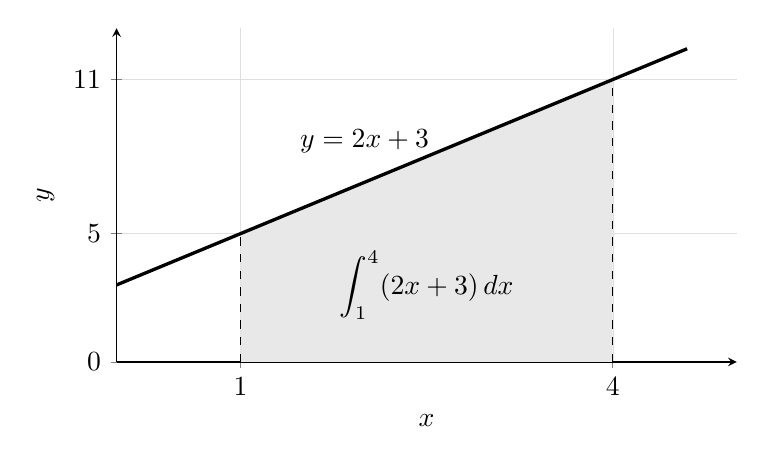
\begin{tikzpicture}
\begin{axis}[
    width=0.78\textwidth,
    height=0.48\textwidth,
    xmin=0, xmax=5,
    ymin=0, ymax=13,
    axis lines=left,
    xlabel={\(x\)},
    ylabel={\(y\)},
    xtick={1,4},
    ytick={0,5,11},
    grid=both,
    grid style={line width=.1pt, draw=gray!25},
]
\addplot[domain=1:4, samples=2, fill=gray!18, draw=none] {2*x+3} \closedcycle;
\addplot[very thick, domain=0:4.6, samples=2] {2*x+3};
\draw[dashed] (axis cs:1,0) -- (axis cs:1,5);
\draw[dashed] (axis cs:4,0) -- (axis cs:4,11);
\node[anchor=center] at (axis cs:2.0,8.6) {\(y=2x+3\)};
\node at (axis cs:2.5,3.0) {\(\displaystyle\int_1^4(2x+3)\,dx\)};
\end{axis}
\end{tikzpicture}
\caption{The integral of \(2x+3\) from \(1\) to \(4\) is the area of a trapezoid.}
\label{fig:ftc2-line-area}
\end{figure}

Now compute the same number with an antiderivative.

A function whose derivative is

\[
2x+3
\]

is

\[
F(x)=x^2+3x,
\]

because

\[
F'(x)=2x+3.
\]

Evaluate \(F\) at the endpoints:

\[
F(4)=4^2+3(4)=28,
\]

and

\[
F(1)=1^2+3(1)=4.
\]

Subtract:

\[
F(4)-F(1)=28-4=24.
\]

This matches the trapezoid area:

\[
\boxed{
\int_1^4(2x+3)\,dx=F(4)-F(1).
}
\]

The antiderivative has turned an accumulation problem into an endpoint calculation.

\begin{quote}
\textbf{The pattern.}
If \(F'(x)=f(x)\), then

\[
\int_a^b f(x)\,dx
\]

should equal the total change in \(F\) from \(a\) to \(b\):

\[
F(b)-F(a).
\]
\end{quote}

This is the second part of the Fundamental Theorem of Calculus.

\subsection{The statement of Part II}
\label{subsec:statement-ftc2}

\begin{quote}
\textbf{Fundamental Theorem of Calculus, Part II.}
Let \(f\) be continuous on \([a,b]\).  Suppose \(F\) is an antiderivative of \(f\) on an
interval containing \([a,b]\); that is,

\[
F'(x)=f(x)
\]

for every \(x\) in that interval.  Then

\[
\boxed{
\int_a^b f(x)\,dx=F(b)-F(a).
}
\]
\end{quote}

We often write the endpoint subtraction as

\[
F(x)\Big|_a^b=F(b)-F(a).
\]

So Part II can be written compactly as

\[
\boxed{
\int_a^b f(x)\,dx=F(x)\Big|_a^b.
}
\]

The notation \(F(x)\big|_a^b\) means:

\[
\text{evaluate at the top endpoint, evaluate at the bottom endpoint, subtract.}
\]

\paragraph{Example.}
Evaluate

\[
\int_0^3 x^2\,dx.
\]

An antiderivative of \(x^2\) is

\[
F(x)=\frac{x^3}{3}.
\]

Therefore

\[
\int_0^3 x^2\,dx
=
\frac{x^3}{3}\Big|_0^3
=
\frac{3^3}{3}-\frac{0^3}{3}
=
9.
\]

So

\[
\boxed{
\int_0^3 x^2\,dx=9.
}
\]

\paragraph{Example.}
Evaluate

\[
\int_1^2 (x^3-4x+1)\,dx.
\]

An antiderivative is

\[
F(x)=\frac{x^4}{4}-2x^2+x.
\]

Thus

\[
\int_1^2 (x^3-4x+1)\,dx
=
\left(\frac{x^4}{4}-2x^2+x\right)\Big|_1^2.
\]

Compute the endpoint values:

\[
F(2)=\frac{16}{4}-2(4)+2=4-8+2=-2,
\]

and

\[
F(1)=\frac14-2+1=-\frac34.
\]

Therefore

\[
\int_1^2 (x^3-4x+1)\,dx
=
-2-\left(-\frac34\right)
=
-\frac54.
\]

So

\[
\boxed{
\int_1^2 (x^3-4x+1)\,dx=-\frac54.
}
\]

The answer is negative because the signed area below the axis exceeds the signed area
above the axis on this interval.

\subsection{Proof of Part II}
\label{subsec:proof-ftc2}

The proof is short because Part I already did the hard work.

\paragraph{Proof.}
Define the accumulation function

\[
A(x)=\int_a^x f(t)\,dt.
\]

By Part I,

\[
A'(x)=f(x).
\]

We are also given that

\[
F'(x)=f(x).
\]

Therefore

\[
A'(x)=F'(x).
\]

So

\[
(A-F)'(x)=0.
\]

A function whose derivative is \(0\) throughout an interval is constant on that interval.
Hence

\[
A(x)-F(x)=C
\]

for some constant \(C\).

Now use \(x=a\).  Since

\[
A(a)=\int_a^a f(t)\,dt=0,
\]

we get

\[
0-F(a)=C.
\]

Thus

\[
C=-F(a).
\]

Therefore

\[
A(x)-F(x)=-F(a),
\]

or

\[
A(x)=F(x)-F(a).
\]

Finally put \(x=b\):

\[
\int_a^b f(t)\,dt
=
A(b)
=
F(b)-F(a).
\]

The letter inside the integral is a placeholder, so we may write

\[
\int_a^b f(x)\,dx=F(b)-F(a).
\]

This proves Part II. \(\square\)

\subsection{Why the interval hypothesis matters}
\label{subsec:ftc2-interval-hypothesis}

Part II requires one antiderivative on an interval containing the whole interval of
integration.  We cannot use an antiderivative formula across a break where the function
is not defined.

For example, consider

\[
f(x)=\frac1{x^2}.
\]

A formal antiderivative is

\[
F(x)=-\frac1x,
\]

because

\[
F'(x)=\frac1{x^2}.
\]

But this formula is valid only on intervals that do not cross \(0\), such as \((0,\infty)\)
or \((-\infty,0)\).  It is not an antiderivative on \([-1,1]\), because \(f\) is not even
defined at \(0\).

If we blindly wrote

\[
\int_{-1}^1 \frac1{x^2}\,dx
=
-\frac1x\Big|_{-1}^{1},
\]

we would get

\[
-1-1=-2.
\]

That is impossible for a positive function.  The real problem is that the integral is not
a proper definite integral on \([-1,1]\).  The function blows up at \(0\), and Part II does
not apply.

\begin{quote}
\textbf{Moral.}
Endpoint subtraction is allowed only when the antiderivative is valid on one interval
covering the whole trip from \(a\) to \(b\).
\end{quote}

This warning will return when we study improper integrals.  For now, the safe rule is:

\[
\boxed{
\text{Check that the integrand is continuous on the interval before using Part II.}
}
\]

\subsection{The net change theorem}
\label{subsec:net-change-theorem}

Part II is often most meaningful when the integrand is a derivative.

If

\[
F'(x)=f(x),
\]

then

\[
\int_a^b f(x)\,dx
=
F(b)-F(a).
\]

Replacing \(f\) by \(F'\), we get

\[
\boxed{
\int_a^b F'(x)\,dx=F(b)-F(a).
}
\]

This is called the \emph{net change theorem}.

\begin{quote}
\textbf{Net change theorem.}
The integral of a rate of change gives the net change in the original quantity:

\[
\boxed{
\int_a^b \text{rate of change}\,dx
=
\text{final amount}-\text{initial amount}.
}
\]
\end{quote}

The word \emph{net} matters.  Positive and negative changes can cancel.

\paragraph{Example: temperature change.}
Suppose the temperature of a metal plate changes at the rate

\[
T'(t)=6-2t
\]

degrees Celsius per minute, for

\[
0\le t\le5.
\]

Find the net temperature change from \(t=0\) to \(t=5\).

By the net change theorem,

\[
T(5)-T(0)=\int_0^5 (6-2t)\,dt.
\]

An antiderivative of \(6-2t\) is

\[
6t-t^2.
\]

So

\[
\int_0^5 (6-2t)\,dt
=
(6t-t^2)\Big|_0^5
=
(30-25)-0
=
5.
\]

The net temperature change is

\[
\boxed{5^\circ\text{C}.}
\]

The rate \(T'(t)\) becomes negative after \(t=3\).  So the temperature first rises, then
falls.  The integral counts both effects with signs.

\subsection{Position from velocity}
\label{subsec:position-from-velocity-ftc2}

The dashboard story now becomes a theorem.

If \(s(t)\) is position and \(v(t)=s'(t)\) is velocity, then

\[
\boxed{
\int_a^b v(t)\,dt=s(b)-s(a).
}
\]

The integral of velocity is displacement.

\paragraph{Example: displacement and distance are different.}
A particle has velocity

\[
v(t)=3t^2-12t+9
=
3(t-1)(t-3),
\qquad 0\le t\le4.
\]

Find its displacement from \(0\) to \(4\).  Then find the total distance traveled.

An antiderivative of \(v(t)\) is

\[
s(t)=t^3-6t^2+9t.
\]

So the displacement is

\[
\int_0^4 v(t)\,dt
=
s(4)-s(0).
\]

Compute:

\[
s(4)=64-96+36=4,
\qquad
s(0)=0.
\]

Thus

\[
\boxed{
\int_0^4 v(t)\,dt=4.
}
\]

The displacement is \(4\) units.

But total distance traveled counts all motion as positive.  The velocity factors as

\[
v(t)=3(t-1)(t-3),
\]

so \(v(t)\) changes sign at

\[
t=1
\qquad\text{and}\qquad
t=3.
\]

It is positive on \([0,1]\), negative on \([1,3]\), and positive on \([3,4]\).

The position values are

\[
s(0)=0,
\qquad
s(1)=1-6+9=4,
\]

\[
s(3)=27-54+27=0,
\qquad
s(4)=4.
\]

Therefore the total distance traveled is

\[
|s(1)-s(0)|+|s(3)-s(1)|+|s(4)-s(3)|.
\]

So

\[
\text{total distance}
=
|4-0|+|0-4|+|4-0|
=
4+4+4
=
12.
\]

The displacement is \(4\).  The distance traveled is \(12\).

\begin{figure}[h]
\centering
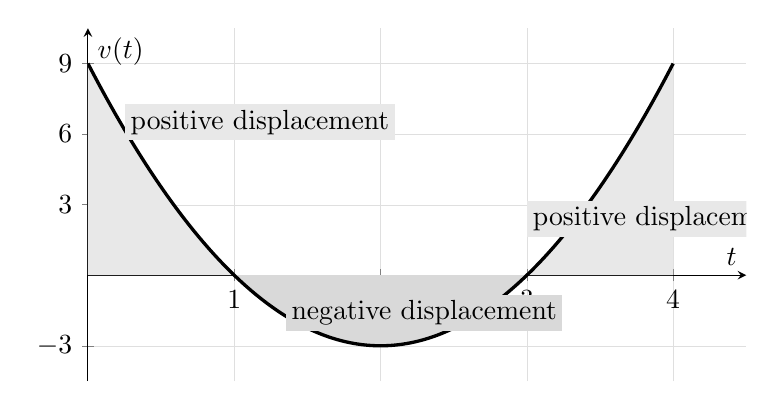
\begin{tikzpicture}
\begin{axis}[
    width=0.82\textwidth,
    height=0.50\textwidth,
    xmin=0, xmax=4.5,
    ymin=-4.5, ymax=10.5,
    axis lines=middle,
    xlabel={\(t\)},
    ylabel={\(v(t)\)},
    xtick={0,1,2,3,4},
    ytick={-3,0,3,6,9},
    grid=both,
    grid style={line width=.1pt, draw=gray!25},
]
\addplot[domain=0:1, samples=80, fill=gray!18, draw=none] {3*(x-1)*(x-3)} \closedcycle;
\addplot[domain=1:3, samples=100, fill=gray!30, draw=none] {3*(x-1)*(x-3)} \closedcycle;
\addplot[domain=3:4, samples=80, fill=gray!18, draw=none] {3*(x-1)*(x-3)} \closedcycle;
\addplot[very thick, domain=0:4, samples=200] {3*(x-1)*(x-3)};

% Added matching fills and inner sep
\node[anchor=west, fill=gray!18, inner sep=2pt] at (axis cs:0.25,6.5) {positive displacement};
\node[anchor=west, fill=gray!30, inner sep=2pt] at (axis cs:1.35,-1.6) {negative displacement};
\node[anchor=west, fill=gray!18, inner sep=2pt] at (axis cs:3.0,2.4) {positive displacement};
\end{axis}
\end{tikzpicture}
\caption{Signed velocity gives displacement.  Total distance requires adding the absolute changes.}
\label{fig:velocity-net-change-sign}
\end{figure}

In integral notation,

\[
\text{displacement}=\int_0^4 v(t)\,dt,
\]

while

\[
\text{total distance}=\int_0^4 |v(t)|\,dt.
\]

The first integral allows cancellation.  The second does not.

\subsection{Accumulated rate in science and economics}
\label{subsec:accumulated-rate-science-economics}

Whenever a quantity is given by a rate, integration recovers accumulated change.

\[
\begin{array}{c|c|c}
\textbf{rate} & \textbf{integral} & \textbf{accumulated quantity} \\ \hline
v(t)\text{ velocity} & \displaystyle\int_a^b v(t)\,dt & \text{displacement} \\[8pt]
P(t)\text{ power} & \displaystyle\int_a^b P(t)\,dt & \text{energy used} \\[8pt]
r(t)\text{ population growth rate} & \displaystyle\int_a^b r(t)\,dt & \text{population change} \\[8pt]
C'(q)\text{ marginal cost} & \displaystyle\int_a^b C'(q)\,dq & \text{cost increase}
\end{array}
\]

The units confirm the meaning.

\[
\text{kW}\cdot\text{hours}=\text{kWh},
\]

so the integral of power over time is energy.

\[
\frac{\text{dollars}}{\text{item}}\cdot\text{items}=\text{dollars},
\]

so the integral of marginal cost over quantity is a change in cost.

\paragraph{Example: energy from power.}
A machine uses power

\[
P(t)=0.5+0.1t
\]

kilowatts \(t\) hours after it is turned on.  How much energy does it use during the first
\(4\) hours?

Energy is accumulated power:

\[
E=\int_0^4 P(t)\,dt.
\]

So

\[
E=\int_0^4 (0.5+0.1t)\,dt.
\]

An antiderivative is

\[
0.5t+0.05t^2.
\]

Therefore

\[
E=
(0.5t+0.05t^2)\Big|_0^4
=
2+0.8
=
2.8.
\]

The machine uses

\[
\boxed{2.8\text{ kWh}}
\]

of energy.

\paragraph{Example: marginal cost.}
Suppose the marginal cost of producing the \(q\)th item is modeled by

\[
C'(q)=5+0.02q
\]

dollars per item.  Find the increase in cost when production rises from \(100\) items
to \(160\) items.

The cost increase is

\[
C(160)-C(100)=\int_{100}^{160} C'(q)\,dq.
\]

Thus

\[
C(160)-C(100)
=
\int_{100}^{160} (5+0.02q)\,dq.
\]

An antiderivative is

\[
5q+0.01q^2.
\]

So

\[
C(160)-C(100)
=
(5q+0.01q^2)\Big|_{100}^{160}.
\]

Compute:

\[
5(160)+0.01(160)^2=800+256=1056,
\]

and

\[
5(100)+0.01(100)^2=500+100=600.
\]

Therefore

\[
C(160)-C(100)=1056-600=456.
\]

The cost increases by

\[
\boxed{\$456.}
\]

\begin{quote}
\textbf{Reading Part II in words.}
If \(F\) accumulates \(f\), then \(f\) is the rate of change of \(F\).  The integral of \(f\)
from \(a\) to \(b\) gives the change in \(F\) from \(a\) to \(b\).
\end{quote}

Part II gives a practical method for definite integrals, but it depends on a new skill:
finding antiderivatives.

That skill becomes its own language.

\section{Indefinite integrals}
\label{sec:indefinite-integrals}

Part II says that definite integrals can be evaluated by antiderivatives:

\[
\int_a^b f(x)\,dx=F(b)-F(a),
\qquad F'=f.
\]

So integration now has two faces.

One face is accumulation:

\[
\int_a^b f(x)\,dx.
\]

This is a number.

The other face is antiderivatives:

\[
\text{find all functions }F\text{ such that }F'=f.
\]

That second task needs notation.

\subsection{Antiderivative families}
\label{subsec:antiderivative-families}

The derivative of

\[
\frac{x^3}{3}
\]

is

\[
x^2.
\]

But the derivative of

\[
\frac{x^3}{3}+7
\]

is also

\[
x^2.
\]

The derivative of

\[
\frac{x^3}{3}-100
\]

is still

\[
x^2.
\]

A derivative forgets vertical shifts.  So an antiderivative is never alone.  It comes in a
family.

\[
\frac{x^3}{3}+C,
\]

where \(C\) is any constant, is the whole family of antiderivatives of \(x^2\) on the real
line.

\begin{figure}[h]
\centering
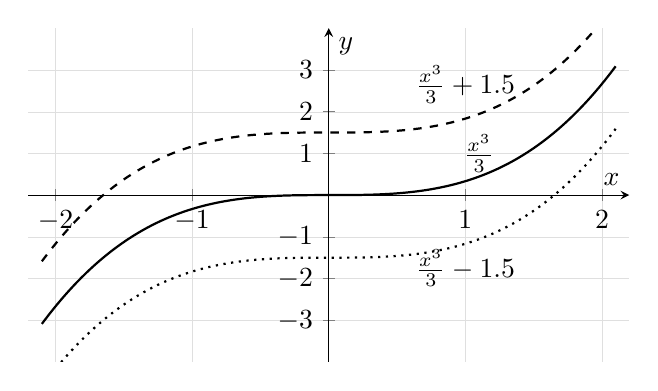
\begin{tikzpicture}
\begin{axis}[
    width=0.76\textwidth,
    height=0.48\textwidth,
    xmin=-2.2, xmax=2.2,
    ymin=-4, ymax=4,
    axis lines=middle,
    xlabel={\(x\)},
    ylabel={\(y\)},
    xtick={-2,-1,0,1,2},
    ytick={-3,-2,-1,0,1,2,3},
    grid=both,
    grid style={line width=.1pt, draw=gray!25},
]
\addplot[thick, domain=-2.1:2.1, samples=200] {x^3/3};
\addplot[thick, dashed, domain=-2.1:2.1, samples=200] {x^3/3+1.5};
\addplot[thick, dotted, domain=-2.1:2.1, samples=200] {x^3/3-1.5};
\node[anchor=center] at (axis cs:1.1,1.0) {\(\frac{x^3}{3}\)};
\node[anchor=center] at (axis cs:1.0,2.65) {\(\frac{x^3}{3}+1.5\)};
\node[anchor=center] at (axis cs:1.0,-1.75) {\(\frac{x^3}{3}-1.5\)};
\end{axis}
\end{tikzpicture}
\caption{Antiderivatives of the same function differ by vertical shifts.  Their slopes at the same \(x\)-value are equal.}
\label{fig:antiderivative-family-shifts}
\end{figure}

\begin{quote}
\textbf{Indefinite integral.}
The notation

\[
\boxed{
\int f(x)\,dx
}
\]

means the family of all antiderivatives of \(f\).  If \(F'(x)=f(x)\), then

\[
\boxed{
\int f(x)\,dx=F(x)+C.
}
\]

The constant \(C\) is called the \emph{constant of integration}.
\end{quote}

For example,

\[
\boxed{
\int x^2\,dx=\frac{x^3}{3}+C.
}
\]

The symbol \(dx\) still matters.  It says that \(x\) is the variable of integration.  It also
prepares the substitution rules we will need next.

\paragraph{Definite versus indefinite.}
A definite integral has limits:

\[
\int_a^b f(x)\,dx.
\]

It is a number.

An indefinite integral has no limits:

\[
\int f(x)\,dx.
\]

It is a family of functions.

\[
\boxed{
\text{Definite integral: number.}
\qquad
\text{Indefinite integral: family of antiderivatives.}
}
\]

\subsection{The constant of integration}
\label{subsec:constant-of-integration}

Why do we write \(+C\)?

Because all functions with the same derivative differ by a constant, as long as we are
working on one interval.

\begin{quote}
\textbf{Same derivative, same up to a constant.}
If \(F\) and \(G\) are differentiable on an interval \(I\), and

\[
F'(x)=G'(x)
\]

for every \(x\in I\), then

\[
F(x)=G(x)+C
\]

for some constant \(C\).
\end{quote}

\paragraph{Proof.}
Let

\[
H(x)=F(x)-G(x).
\]

Then

\[
H'(x)=F'(x)-G'(x)=0.
\]

By the Mean Value Theorem, if \(x_1\) and \(x_2\) are any two points in the interval,
then for some \(c\) between them,

\[
\frac{H(x_2)-H(x_1)}{x_2-x_1}=H'(c)=0.
\]

So

\[
H(x_2)-H(x_1)=0,
\]

which means

\[
H(x_2)=H(x_1).
\]

Thus \(H\) is constant on the interval.  Therefore

\[
F(x)-G(x)=C,
\]

or

\[
F(x)=G(x)+C.
\]

\paragraph{Why ``on an interval'' matters.}
The interval condition is not decoration.

Define

\[
H(x)=
\begin{cases}
0, & x<0,\\
1, & x>0.
\end{cases}
\]

The domain is

\[
(-\infty,0)\cup(0,\infty).
\]

On this domain, the derivative is

\[
H'(x)=0
\]

at every point where \(H\) is defined.  But \(H\) is not one constant on its whole domain.
It is \(0\) on the left interval and \(1\) on the right interval.

The conclusion ``derivative zero means constant'' works on intervals, because intervals
are connected pieces of the line.

This is why formulas such as

\[
\int \frac1x\,dx=\ln|x|+C
\]

must be understood on intervals that do not cross \(0\).  On \((0,\infty)\),

\[
\ln|x|=\ln x.
\]

On \((-\infty,0)\),

\[
\ln|x|=\ln(-x).
\]

The two sides are separate intervals.

\subsection{Initial value problems}
\label{subsec:initial-value-problems-antiderivatives}

An indefinite integral gives a family.  A starting value chooses one member of the
family.

\paragraph{Example: position from velocity and one position value.}
A particle has velocity

\[
v(t)=6t-4
\]

meters per second.  Its position at \(t=1\) is

\[
s(1)=10.
\]

Find \(s(t)\).

Since

\[
s'(t)=v(t)=6t-4,
\]

we first find the general antiderivative:

\[
s(t)=\int (6t-4)\,dt.
\]

Compute:

\[
s(t)=3t^2-4t+C.
\]

Now use the initial value:

\[
s(1)=3(1)^2-4(1)+C=10.
\]

So

\[
3-4+C=10,
\]

hence

\[
C=11.
\]

Therefore

\[
\boxed{
s(t)=3t^2-4t+11.
}
\]

The velocity gives the shape of the position function.  The initial position fixes its
vertical placement.

\begin{quote}
\textbf{Initial value problem.}
A problem of the form

\[
F'(x)=f(x),
\qquad
F(a)=F_0
\]

asks for the particular antiderivative of \(f\) that passes through the point
\((a,F_0)\).
\end{quote}

\paragraph{Example.}
Solve

\[
y'=3x^2-2x,
\qquad
y(0)=5.
\]

First integrate:

\[
y=\int (3x^2-2x)\,dx.
\]

So

\[
y=x^3-x^2+C.
\]

Use \(y(0)=5\):

\[
5=0^3-0^2+C,
\]

so

\[
C=5.
\]

Thus

\[
\boxed{
y=x^3-x^2+5.
}
\]

This is the simplest kind of differential equation.  Later, differential equations will be
harder because the derivative will depend on the unknown function itself.  But the
first case is already clear: integrating a derivative gives a family, and an initial value
selects one function.

\subsection{Basic antiderivative formulas}
\label{subsec:basic-antiderivative-formulas}

Every antiderivative formula can be checked by differentiating the right-hand side.

The first formulas reverse the derivative rules we already know.

\[
\begin{array}{c|c}
\textbf{integrand} & \textbf{indefinite integral} \\ \hline
0 & \displaystyle C \\[6pt]
k & \displaystyle kx+C \\[6pt]
x^n,\ n\neq -1 & \displaystyle \frac{x^{n+1}}{n+1}+C \\[10pt]
\dfrac1x & \displaystyle \ln|x|+C \\[10pt]
e^x & \displaystyle e^x+C \\[6pt]
a^x,\ a>0,\ a\neq1 & \displaystyle \frac{a^x}{\ln a}+C
\end{array}
\]

The power rule for antiderivatives deserves special attention:

\[
\boxed{
\int x^n\,dx=\frac{x^{n+1}}{n+1}+C,
\qquad n\neq -1.
}
\]

The case \(n=-1\) is excluded because it would require division by \(0\).  That case is

\[
\int \frac1x\,dx=\ln|x|+C.
\]

The trigonometric formulas reverse the trigonometric derivative formulas.

\[
\begin{array}{c|c}
\textbf{integrand} & \textbf{indefinite integral} \\ \hline
\cos x & \displaystyle \sin x+C \\[6pt]
\sin x & \displaystyle -\cos x+C \\[6pt]
\sec^2 x & \displaystyle \tan x+C \\[6pt]
\csc^2 x & \displaystyle -\cot x+C \\[6pt]
\sec x\tan x & \displaystyle \sec x+C \\[6pt]
\csc x\cot x & \displaystyle -\csc x+C
\end{array}
\]

And the inverse-trigonometric derivative formulas give

\[
\begin{array}{c|c}
\textbf{integrand} & \textbf{indefinite integral} \\ \hline
\dfrac1{1+x^2} & \displaystyle \arctan x+C \\[12pt]
\dfrac1{\sqrt{1-x^2}} & \displaystyle \arcsin x+C
\end{array}
\]

These formulas are not separate magic.  They are derivative facts read backward.

\paragraph{Example: polynomial and trigonometric terms.}
Find

\[
\int (4x^3-6x+2\cos x)\,dx.
\]

Use linearity:

\[
\int (4x^3-6x+2\cos x)\,dx
=
4\int x^3\,dx
-
6\int x\,dx
+
2\int \cos x\,dx.
\]

Thus

\[
=4\left(\frac{x^4}{4}\right)
-
6\left(\frac{x^2}{2}\right)
+
2\sin x
+
C.
\]

So

\[
\boxed{
\int (4x^3-6x+2\cos x)\,dx
=
x^4-3x^2+2\sin x+C.
}
\]

Check by differentiating:

\[
\frac{d}{dx}(x^4-3x^2+2\sin x+C)
=
4x^3-6x+2\cos x.
\]

\paragraph{Example: using the logarithm case.}
Find

\[
\int \left(\frac3x+2e^x\right)\,dx.
\]

Use the formulas:

\[
\int \frac3x\,dx=3\ln|x|,
\]

and

\[
\int 2e^x\,dx=2e^x.
\]

Therefore

\[
\boxed{
\int \left(\frac3x+2e^x\right)\,dx
=
3\ln|x|+2e^x+C.
}
\]

This formula is valid on any interval that does not contain \(0\).

\paragraph{Example: a definite integral using an indefinite integral.}
Evaluate

\[
\int_0^{\pi/2} (2\sin x+\cos x)\,dx.
\]

First find an antiderivative:

\[
\int (2\sin x+\cos x)\,dx
=
-2\cos x+\sin x+C.
\]

For the definite integral, the constant cancels, so we use

\[
F(x)=-2\cos x+\sin x.
\]

Then

\[
\int_0^{\pi/2} (2\sin x+\cos x)\,dx
=
F(x)\Big|_0^{\pi/2}.
\]

Compute:

\[
F\left(\frac{\pi}{2}\right)
=
-2\cos\frac{\pi}{2}+\sin\frac{\pi}{2}
=
0+1=1,
\]

and

\[
F(0)=-2\cos0+\sin0=-2.
\]

Therefore

\[
\int_0^{\pi/2} (2\sin x+\cos x)\,dx
=
1-(-2)=3.
\]

So

\[
\boxed{
\int_0^{\pi/2} (2\sin x+\cos x)\,dx=3.
}
\]

\subsection{Linearity of indefinite integrals}
\label{subsec:linearity-indefinite-integrals}

Since derivatives are linear, antiderivatives are linear too.

If \(a\) and \(b\) are constants, then

\[
\boxed{
\int \bigl(a f(x)+b g(x)\bigr)\,dx
=
a\int f(x)\,dx+b\int g(x)\,dx.
}
\]

This formula is useful, but it should be read carefully.  Each indefinite integral already
contains an arbitrary constant.  In practice, we combine all constants into one \(C\).

For example,

\[
\int (3x^2+5)\,dx
=
3\int x^2\,dx+\int 5\,dx.
\]

One could write

\[
3\left(\frac{x^3}{3}+C_1\right)+(5x+C_2).
\]

This equals

\[
x^3+5x+(3C_1+C_2).
\]

Since

\[
3C_1+C_2
\]

is just another arbitrary constant, we write

\[
\boxed{
\int (3x^2+5)\,dx=x^3+5x+C.
}
\]

Use one \(C\) at the end.

\subsection{When guessing is not enough}
\label{subsec:when-guessing-antiderivatives-not-enough}

The formulas above give a starting library.  They do not solve every integral.

For example,

\[
\int 2x\cos(x^2)\,dx
\]

does not appear directly in the table.  But it has a hidden structure.  The inside function

\[
x^2
\]

has derivative

\[
2x,
\]

and that factor is present.  Since

\[
\frac{d}{dx}\sin(x^2)=2x\cos(x^2),
\]

we get

\[
\int 2x\cos(x^2)\,dx=\sin(x^2)+C.
\]

This example is a reverse chain rule.

But if the integral were

\[
\int \cos(x^2)\,dx,
\]

the helpful factor \(2x\) would be missing.  That integral has no elementary
antiderivative.  Part I still guarantees that

\[
\int_0^x \cos(t^2)\,dt
\]

is a real function with derivative \(\cos(x^2)\).  It simply cannot be written using the
basic elementary formulas we know.

So antiderivatives have two sides:

\[
\text{existence}
\qquad\text{and}\qquad
\text{finding a usable formula}.
\]

Part I gives existence for continuous functions.  Part II turns usable formulas into
definite integrals.  The next question is how to find more usable formulas by reversing
the chain rule.

\section{Differential notation and oriented length}
\label{sec:differential-notation-oriented-length}

Substitution gave us a powerful rule:

\[
\int f(g(u))g'(u)\,du.
\]

At first this may look like a trick with symbols.  But the symbols are trying to say
something geometric.

When

\[
x=g(u),
\]

a small step in \(u\) produces a small step in \(x\):

\[
dx=g'(u)\,du.
\]

So the expression

\[
f(x)\,dx
\]

is not just a function \(f(x)\) with decoration attached.  It is the small accumulated
amount:

\[
\text{height}\times\text{oriented width}.
\]

This section slows down the notation so that later formulas feel less mysterious.

\subsection{\texorpdfstring{\(dx\)}{dx} as an oriented step}
\label{subsec:dx-oriented-step}

The definite integral

\[
\int_a^b f(x)\,dx
\]

accumulates from \(a\) to \(b\).  The direction matters.

If \(a<b\), we move left to right.  A small step \(dx\) is positive.

If \(b<a\), we move right to left.  A small step \(dx\) is negative.

That is why

\[
\boxed{
\int_b^a f(x)\,dx=-\int_a^b f(x)\,dx.
}
\]

The symbol \(dx\) carries the direction of traversal.

\begin{figure}[h]
\centering
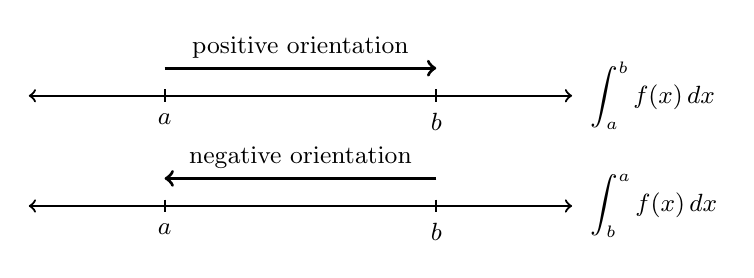
\begin{tikzpicture}[xscale=1.15, every node/.style={font=\small}]
  % first line
  \draw[<->, thick] (-0.5,1.4) -- (5.5,1.4);
  \foreach \x/\lab in {1/a,4/b} {
    \draw[thick] (\x,1.48) -- (\x,1.32);
    \node[below] at (\x,1.3) {\(\lab\)};
  }
  \draw[very thick, ->] (1,1.75) -- (4,1.75);
  \node[above] at (2.5,1.75) {positive orientation};
  \node[right] at (5.6,1.4) {\(\displaystyle\int_a^b f(x)\,dx\)};

  % second line
  \draw[<->, thick] (-0.5,0) -- (5.5,0);
  \foreach \x/\lab in {1/a,4/b} {
    \draw[thick] (\x,0.08) -- (\x,-0.08);
    \node[below] at (\x,-0.1) {\(\lab\)};
  }
  \draw[very thick, ->] (4,0.35) -- (1,0.35);
  \node[above] at (2.5,0.35) {negative orientation};
  \node[right] at (5.6,0) {\(\displaystyle\int_b^a f(x)\,dx\)};
\end{tikzpicture}
\caption{The same interval with opposite orientations gives integrals with opposite signs.}
\label{fig:oriented-interval}
\end{figure}

The simplest example is the integral of \(1\).

If we move from \(2\) to \(5\), then

\[
\int_2^5 1\,dx=5-2=3.
\]

If we move from \(5\) to \(2\), then

\[
\int_5^2 1\,dx=2-5=-3.
\]

So

\[
\int_a^b 1\,dx=b-a.
\]

This is \emph{oriented length}.  Ordinary length is always positive:

\[
\text{ordinary length of }[a,b]=|b-a|.
\]

But the integral remembers direction:

\[
\boxed{
\text{oriented length from \(a\) to \(b\) is }b-a.
}
\]

\paragraph{Example.}
Compute

\[
\int_4^1 3\,dx.
\]

Since the integrand is constant,

\[
\int_4^1 3\,dx=3(1-4)=-9.
\]

The ordinary area of the rectangle would be

\[
3\cdot3=9.
\]

The integral is negative because the traversal is from right to left.

\subsection{\texorpdfstring{\(f(x)\,dx\)}{f(x) dx} as the thing being accumulated}
\label{subsec:integrand-being-accumulated}

A Riemann sum has terms of the form

\[
f(x_i^*)\Delta x_i.
\]

Each term is

\[
\text{sampled height}\times\text{small oriented width}.
\]

The integral is the limit of such sums:

\[
\int_a^b f(x)\,dx.
\]

So the expression

\[
f(x)\,dx
\]

should be read as one unit:

\[
\boxed{
f(x)\,dx=\text{a small signed amount to be accumulated.}
}
\]

The function \(f(x)\) supplies the density, rate, or height.  The \(dx\) supplies the
oriented step along the \(x\)-axis.

This is why units work naturally.

\[
\begin{array}{c|c|c}
\textbf{integrand} & \textbf{units} & \textbf{accumulated quantity} \\ \hline
v(t)\,dt & \dfrac{\text{miles}}{\text{hour}}\cdot\text{hour} & \text{miles} \\[10pt]
\rho(x)\,dx & \dfrac{\text{grams}}{\text{cm}}\cdot\text{cm} & \text{grams} \\[10pt]
P(t)\,dt & \text{kW}\cdot\text{hour} & \text{kWh}
\end{array}
\]

The \(dx\) is part of the meaning of the integral.

\paragraph{Example: mass of a rod.}
Suppose a thin rod lies along the \(x\)-axis from \(x=1\) to \(x=4\).  Its linear density is

\[
\rho(x)=2+x
\]

grams per centimeter.  The small mass near \(x\) is approximately

\[
\rho(x)\,dx=(2+x)\,dx.
\]

Therefore the total mass is

\[
\int_1^4 (2+x)\,dx.
\]

An antiderivative is

\[
2x+\frac{x^2}{2}.
\]

Thus

\[
\int_1^4 (2+x)\,dx
=
\left(2x+\frac{x^2}{2}\right)\Big|_1^4.
\]

Compute:

\[
\left(8+\frac{16}{2}\right)-\left(2+\frac12\right)
=
16-\frac52
=
\frac{27}{2}.
\]

So the mass is

\[
\boxed{\frac{27}{2}\text{ grams}.}
\]

If we wrote

\[
\int_4^1 (2+x)\,dx,
\]

the answer would be

\[
-\frac{27}{2}.
\]

That negative value is not a negative physical mass.  It is the oriented accumulation
from \(4\) back to \(1\).  For physical mass, we choose the natural left-to-right
orientation or take ordinary length.

\begin{quote}
\textbf{Moral.}
The definite integral records both size and direction.  Applications decide whether
that signed quantity is the desired physical quantity.
\end{quote}

\subsection{Pulling an integrand through \texorpdfstring{\(x=g(u)\)}{x=g(u)}}
\label{subsec:pulling-integrand-through-change}

Substitution is the same idea written in a new coordinate.

Suppose

\[
x=g(u).
\]

Then a small change in \(u\) produces a small change in \(x\):

\[
dx=g'(u)\,du.
\]

So the integrand changes by substitution:

\[
\boxed{
f(x)\,dx
=
f(g(u))g'(u)\,du.
}
\]

This is not blind symbol pushing.  It says:

\[
\text{old height}\times\text{old step}
=
\text{new height}\times\text{new step}.
\]

The factor \(g'(u)\) converts a step in \(u\) into the corresponding oriented step in
\(x\).

\paragraph{Example: stretching the measuring stick.}
Evaluate

\[
\int_0^4 \sqrt{x}\,dx
\]

using the substitution

\[
x=u^2.
\]

As \(x\) goes from \(0\) to \(4\), \(u\) goes from \(0\) to \(2\).  Also,

\[
dx=2u\,du.
\]

Since

\[
\sqrt{x}=\sqrt{u^2}=u
\]

for \(0\le u\le2\), we get

\[
\int_0^4 \sqrt{x}\,dx
=
\int_0^2 u(2u)\,du.
\]

So

\[
\int_0^4 \sqrt{x}\,dx
=
\int_0^2 2u^2\,du
=
2\cdot\frac{u^3}{3}\Big|_0^2
=
\frac{16}{3}.
\]

The substitution did not change the accumulated quantity.  It changed how we
described the small steps.

\begin{figure}[h]
\centering
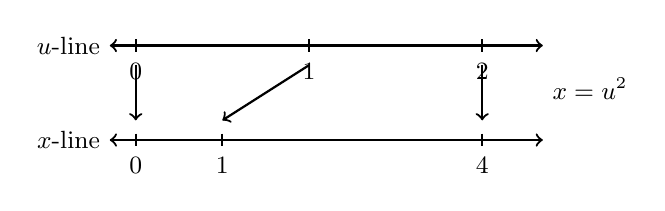
\begin{tikzpicture}[xscale=1.1, every node/.style={font=\small}]
  % u-line
  \draw[<->, thick] (-0.3,1.2) -- (4.7,1.2);
  \foreach \x/\lab in {0/0,2/1,4/2} {
    \draw[thick] (\x,1.28) -- (\x,1.12);
    \node[below] at (\x,1.1) {\(\lab\)};
  }
  \node[left] at (-0.3,1.2) {\(u\)-line};

  % x-line
  \draw[<->, thick] (-0.3,0) -- (4.7,0);
  \foreach \x/\lab in {0/0,1/1,4/4} {
    \draw[thick] (\x,0.08) -- (\x,-0.08);
    \node[below] at (\x,-0.1) {\(\lab\)};
  }
  \node[left] at (-0.3,0) {\(x\)-line};

  % mapping arrows
  \draw[->, thick] (0,0.95) -- (0,0.25);
  \draw[->, thick] (2,0.95) -- (1,0.25);
  \draw[->, thick] (4,0.95) -- (4,0.25);

  \node[right] at (4.7,0.65) {\(x=u^2\)};
\end{tikzpicture}
\caption{The substitution \(x=u^2\) stretches the measuring scale.  Equal \(u\)-steps do not give equal \(x\)-steps.}
\label{fig:substitution-stretching-scale}
\end{figure}

\paragraph{Example: reversed orientation.}
Evaluate

\[
\int_0^1 x^2\,dx
\]

using

\[
x=1-u.
\]

Then

\[
dx=-du.
\]

The limits change too.  When

\[
x=0,
\]

we have

\[
u=1.
\]

When

\[
x=1,
\]

we have

\[
u=0.
\]

Therefore

\[
\int_0^1 x^2\,dx
=
\int_1^0 (1-u)^2(-du).
\]

The negative sign in \(dx=-du\) records the fact that as \(u\) increases, \(x\)
decreases.  We can either keep the negative sign or reverse the limits:

\[
\int_1^0 (1-u)^2(-du)
=
\int_0^1 (1-u)^2\,du.
\]

Thus

\[
\int_0^1 x^2\,dx
=
\int_0^1 (1-u)^2\,du.
\]

Compute:

\[
\int_0^1 (1-u)^2\,du
=
\int_0^1 (1-2u+u^2)\,du
=
\left(u-u^2+\frac{u^3}{3}\right)\Big|_0^1
=
\frac13.
\]

This agrees with

\[
\int_0^1 x^2\,dx=\frac13.
\]

\begin{quote}
\textbf{Substitution rule, read geometrically.}
When \(x=g(u)\),

\[
\int_a^b f(x)\,dx
=
\int_{\alpha}^{\beta} f(g(u))g'(u)\,du,
\]

where

\[
g(\alpha)=a,
\qquad
g(\beta)=b.
\]

The derivative \(g'(u)\) converts \(du\)-steps into oriented \(dx\)-steps.
\end{quote}

The limits are part of the substitution.  They are not decoration.

\subsection{The one-dimensional seed of differential forms}
\label{subsec:one-dimensional-seed-forms}

The notation

\[
f(x)\,dx
\]

has one more future use.  It prepares the language of differential forms.

In one dimension, the basic object that gets accumulated is

\[
f(x)\,dx.
\]

This is a \emph{one-dimensional integrand}.  Later, in multivariable calculus, similar
objects will look like

\[
P(x,y)\,dx+Q(x,y)\,dy.
\]

They will be accumulated along curves.  For now, the one-dimensional case already
contains the main idea:

\[
\boxed{
\text{an integrand is something designed to be integrated along an oriented object.}
}
\]

The most important one-dimensional integrands are exact differentials.

If \(F\) is differentiable, then

\[
dF=F'(x)\,dx.
\]

The Fundamental Theorem, Part II says

\[
\int_a^b F'(x)\,dx=F(b)-F(a).
\]

In differential notation, this becomes

\[
\boxed{
\int_a^b dF=F(b)-F(a).
}
\]

This says:

\[
\text{accumulating the small changes of \(F\)}
=
\text{final value}-\text{initial value}.
\]

The boundary of an oriented interval is its endpoint minus its starting point.  Symbolically,

\[
\partial[a,b]=\{b\}-\{a\}.
\]

So the formula

\[
\int_a^b dF=F(b)-F(a)
\]

can be read as

\[
\text{integral of a derivative over an interval}
=
\text{value on the boundary}.
\]

That sentence will return in multivariable calculus in larger forms.  For now, it is simply
the Fundamental Theorem written in its most compact one-dimensional language.

\paragraph{Example.}
Let

\[
F(x)=x^3-2x.
\]

Then

\[
dF=(3x^2-2)\,dx.
\]

Therefore

\[
\int_1^4 (3x^2-2)\,dx
=
\int_1^4 dF
=
F(4)-F(1).
\]

Compute:

\[
F(4)=64-8=56,
\]

and

\[
F(1)=1-2=-1.
\]

So

\[
\int_1^4 (3x^2-2)\,dx=56-(-1)=57.
\]

The integral accumulated the changes of \(F\) from \(1\) to \(4\).

\subsection{What the notation is allowed to do}
\label{subsec:what-differential-notation-can-do}

Differential notation is powerful when it records a real relationship between small
changes:

\[
dx=g'(u)\,du,
\qquad
dF=F'(x)\,dx.
\]

It is dangerous when it is treated as ordinary multiplication without meaning.

The safe rule is:

\[
\boxed{
\text{Use differential notation to record linear change and oriented accumulation.}
}
\]

For substitution, the notation works because it is the chain rule:

\[
x=g(u)
\quad\Longrightarrow\quad
dx=g'(u)\,du.
\]

For the Fundamental Theorem, the notation works because it is net change:

\[
dF=F'(x)\,dx
\quad\Longrightarrow\quad
\int_a^b dF=F(b)-F(a).
\]

The symbols are compact because the ideas behind them are real.

The next section collects places where these ideas are easy to misuse.  The warnings do
not weaken the formulas.  They make the formulas safer.

\section{Warning examples}
\label{sec:warning-examples-ftc}


This section gathers the most common traps:
\begin{itemize}
    \item a discontinuity in \(f\),
    \item old limits after substitution,
    \item treating an integral like multiplication, and
    \item confusing signed area with ordinary area.
\end{itemize}

A theorem is useful only when we know where it applies.

\subsection{A discontinuity and the derivative of an accumulation function}
\label{subsec:warning-discontinuity-accumulation}

Part I of the Fundamental Theorem said:

\[
A(x)=\int_a^x f(t)\,dt
\quad\Longrightarrow\quad
A'(x)=f(x),
\]

provided \(f\) is continuous.

Continuity matters.

\paragraph{A jump can create a corner.}
Let

\[
f(t)=
\begin{cases}
0, & t<0,\\
1, & t\ge0.
\end{cases}
\]

Define

\[
A(x)=\int_0^x f(t)\,dt.
\]

If \(x<0\), then \(f(t)=0\) on the interval from \(x\) to \(0\), except at one endpoint.
That one point does not affect the integral.  So

\[
A(x)=0
\qquad (x<0).
\]

If \(x>0\), then

\[
A(x)=\int_0^x 1\,dt=x.
\]

Also,

\[
A(0)=0.
\]

Thus

\[
A(x)=
\begin{cases}
0, & x\le0,\\
x, & x>0.
\end{cases}
\]

The graph of \(A\) has a corner at \(0\).  Its left-hand slope is \(0\), and its right-hand
slope is \(1\).  Therefore

\[
A'(0)
\]

does not exist.

\begin{figure}[h]
\centering
\begin{minipage}{0.47\textwidth}
\centering
\begin{tikzpicture}
\begin{axis}[
    width=\textwidth,
    height=0.70\textwidth,
    xmin=-2, xmax=2,
    ymin=-0.25, ymax=1.35,
    axis lines=middle,
    xlabel={\(t\)},
    ylabel={\(f(t)\)},
    xtick={-1,0,1},
    ytick={0,1},
    grid=both,
    grid style={line width=.1pt, draw=gray!25},
    title={jump in \(f\)}
]
\addplot[very thick, domain=-2:-0.03, samples=2] {0};
\addplot[very thick, domain=0.03:2, samples=2] {1};
\addplot[only marks, mark=o, mark size=2.6pt, thick] coordinates {(0,0)};
\addplot[only marks, mark=*, mark size=2.2pt] coordinates {(0,1)};
\end{axis}
\end{tikzpicture}
\end{minipage}
\hfill
\begin{minipage}{0.47\textwidth}
\centering
\begin{tikzpicture}
\begin{axis}[
    width=\textwidth,
    height=0.70\textwidth,
    xmin=-2, xmax=2,
    ymin=-0.25, ymax=2.1,
    axis lines=middle,
    xlabel={\(x\)},
    ylabel={\(A(x)\)},
    xtick={-1,0,1,2},
    ytick={0,1,2},
    grid=both,
    grid style={line width=.1pt, draw=gray!25},
    title={corner in \(A\)}
]
\addplot[very thick, domain=-2:0, samples=2] {0};
\addplot[very thick, domain=0:2, samples=2] {x};
\addplot[only marks, mark=*] coordinates {(0,0)};
\node[anchor=west] at (axis cs:0.0,1.35) {\(A(x)=x\)};
\node[anchor=east] at (axis cs:-0.1,0.25) {\(A(x)=0\)};
\end{axis}
\end{tikzpicture}
\end{minipage}
\caption{A jump discontinuity in \(f\) can produce a corner in the accumulation function \(A\).}
\label{fig:warning-jump-accumulation}
\end{figure}

So the conclusion

\[
A'(0)=f(0)
\]

fails because \(A'(0)\) does not exist.

\paragraph{A one-point discontinuity can make \(A'(c)\neq f(c)\).}
There is an even sharper warning.

Define

\[
f(t)=
\begin{cases}
1, & t=0,\\
0, & t\neq0.
\end{cases}
\]

Let

\[
A(x)=\int_0^x f(t)\,dt.
\]

Changing a function at a single point does not affect its integral.  Therefore

\[
A(x)=0
\]

for every \(x\).  Hence

\[
A'(x)=0
\]

for every \(x\), including \(x=0\).

But

\[
f(0)=1.
\]

Thus

\[
A'(0)=0\neq1=f(0).
\]

The accumulation function is differentiable at \(0\), but its derivative is not equal to
the value of \(f\) at the discontinuity.

\begin{quote}
\textbf{Moral.}
The formula

\[
\frac{d}{dx}\int_a^x f(t)\,dt=f(x)
\]

is guaranteed at points where \(f\) is continuous.  At a discontinuity, the conclusion
can fail in more than one way.
\end{quote}

\subsection{Forgetting the new limits in substitution}
\label{subsec:warning-new-limits-substitution}

A definite integral has endpoints.  When we change variables, the endpoints must
change too.

\paragraph{The mistake.}
Evaluate

\[
\int_1^2 2x\cos(x^2)\,dx.
\]

Let

\[
u=x^2.
\]

Then

\[
du=2x\,dx.
\]

The integrand becomes

\[
\cos u\,du.
\]

A common wrong step is to write

\[
\int_1^2 2x\cos(x^2)\,dx
=
\int_1^2 \cos u\,du.
\]

This keeps the old limits \(1\) and \(2\).  But those were \(x\)-values, not \(u\)-values.

\paragraph{The correction.}
If

\[
u=x^2,
\]

then when

\[
x=1,
\]

we have

\[
u=1.
\]

When

\[
x=2,
\]

we have

\[
u=4.
\]

Therefore

\[
\int_1^2 2x\cos(x^2)\,dx
=
\int_1^4 \cos u\,du.
\]

Now evaluate:

\[
\int_1^4 \cos u\,du
=
\sin u\Big|_1^4
=
\boxed{\sin4-\sin1}.
\]

The wrong limits would give

\[
\sin2-\sin1,
\]

which is not the same.

\begin{quote}
\textbf{Moral.}
In a definite integral, every variable has its own limits.  If \(u=g(x)\), convert the
old \(x\)-limits into new \(u\)-limits.
\end{quote}

\paragraph{A reversed-limit example.}
Evaluate

\[
\int_0^1 2x e^{1-x^2}\,dx.
\]

Let

\[
u=1-x^2.
\]

Then

\[
du=-2x\,dx,
\]

so

\[
2x\,dx=-du.
\]

The limits change:

\[
x=0 \quad\Longrightarrow\quad u=1,
\]

and

\[
x=1 \quad\Longrightarrow\quad u=0.
\]

Therefore

\[
\int_0^1 2x e^{1-x^2}\,dx
=
\int_1^0 e^u(-du).
\]

This equals

\[
\int_0^1 e^u\,du
=
e^u\Big|_0^1
=
\boxed{e-1}.
\]

The negative sign and the reversed limits are two ways of recording the same
orientation change.  They must be handled together, not ignored.

\subsection{Treating \texorpdfstring{\(\int f(x)\,dx\)}{int f(x) dx} like multiplication}
\label{subsec:warning-integral-like-multiplication}

The notation

\[
\int f(x)\,dx
\]

is meaningful, but it is not ordinary multiplication.

The symbol \(\int\) is not a number.  The symbol \(dx\) is not a factor that can be
moved around freely.  Together they describe an operation: find a family of
antiderivatives.

\paragraph{Only constants can be pulled out.}
It is true that

\[
\int c f(x)\,dx=c\int f(x)\,dx
\]

when \(c\) is a constant.

But it is not true that

\[
\int x f(x)\,dx=x\int f(x)\,dx
\]

in general.

\paragraph{A simple false step.}
Suppose someone tries

\[
\int x\,dx
=
x\int 1\,dx
=
x(x+C)
=
x^2+Cx.
\]

This is wrong because \(x\) is not a constant.  It changes with the variable of
integration.

The correct result is

\[
\int x\,dx=\frac{x^2}{2}+C.
\]

We can check by differentiating:

\[
\frac{d}{dx}\left(\frac{x^2}{2}+C\right)=x.
\]

But

\[
\frac{d}{dx}(x^2+Cx)=2x+C,
\]

which is not \(x\) unless by accident at special points.

\begin{quote}
\textbf{Moral.}
An indefinite integral is an instruction to find antiderivatives.  It is linear with
respect to constants and sums, but it is not ordinary multiplication.
\end{quote}

\paragraph{Another common false pattern.}
It is also not true that

\[
\int f(x)g(x)\,dx
=
\left(\int f(x)\,dx\right)
\left(\int g(x)\,dx\right).
\]

For example, take

\[
f(x)=g(x)=1.
\]

Then the left side is

\[
\int 1\cdot1\,dx
=
\int 1\,dx
=
x+C.
\]

But the right side would be

\[
\left(\int 1\,dx\right)\left(\int 1\,dx\right)
=
(x+C_1)(x+C_2),
\]

which is a quadratic expression, not a family of antiderivatives of \(1\).

Linearity is safe:

\[
\int (f+g)\,dx=\int f\,dx+\int g\,dx.
\]

Products require different methods.  They are not handled by multiplying
antiderivatives.

\subsection{Confusing area with net signed area}
\label{subsec:warning-area-net-signed-area}

A definite integral measures signed accumulation.  It is not always ordinary
geometric area.

Consider

\[
\int_{-1}^{1} x\,dx.
\]

An antiderivative of \(x\) is

\[
\frac{x^2}{2}.
\]

So

\[
\int_{-1}^{1} x\,dx
=
\frac{x^2}{2}\Big|_{-1}^{1}
=
\frac12-\frac12
=
0.
\]

The answer is \(0\).  But the graph does enclose visible area with the \(x\)-axis.

The triangle above the axis from \(0\) to \(1\) has area

\[
\frac12.
\]

The triangle below the axis from \(-1\) to \(0\) also has ordinary area

\[
\frac12.
\]

The integral counts the lower triangle as negative, so the two signed areas cancel.

\begin{figure}[h]
\centering
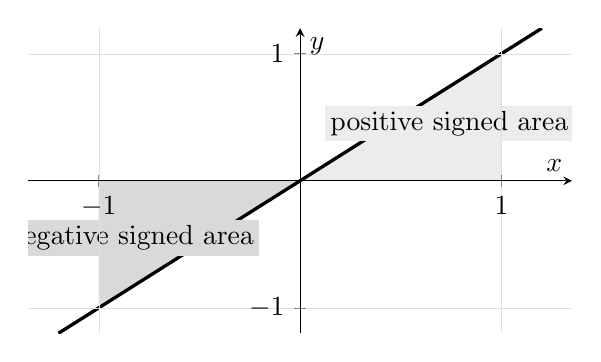
\begin{tikzpicture}
\begin{axis}[
    width=0.70\textwidth,
    height=0.45\textwidth,
    xmin=-1.35, xmax=1.35,
    ymin=-1.2, ymax=1.2,
    axis lines=middle,
    axis on top,
    xlabel={\(x\)},
    ylabel={\(y\)},
    xtick={-1,0,1},
    ytick={-1,0,1},
    grid=both,
    grid style={line width=.1pt, draw=gray!25},
]
\addplot[domain=-1:0, samples=2, fill=gray!30, draw=none] {x} \closedcycle;
\addplot[domain=0:1, samples=2, fill=gray!15, draw=none] {x} \closedcycle;
\addplot[very thick, domain=-1.2:1.2, samples=2] {x};
\node[anchor=east, fill=gray!30, inner sep=2pt] at (axis cs:-0.2,-0.45) {negative signed area};
\node[anchor=west, fill=gray!15, inner sep=2pt] at (axis cs:0.12,0.45) {positive signed area};
\end{axis}
\end{tikzpicture}
\caption{The integral of \(x\) from \(-1\) to \(1\) is zero because positive and negative signed areas cancel.}
\label{fig:signed-area-cancellation-line}
\end{figure}

If we want ordinary geometric area, we integrate the absolute value:

\[
\int_{-1}^{1} |x|\,dx.
\]

This gives

\[
\int_{-1}^{0} (-x)\,dx+\int_0^1 x\,dx.
\]

Compute:

\[
\int_{-1}^{0} (-x)\,dx
=
-\frac{x^2}{2}\Big|_{-1}^{0}
=
0-\left(-\frac12\right)
=
\frac12,
\]

and

\[
\int_0^1 x\,dx
=
\frac12.
\]

So

\[
\int_{-1}^{1}|x|\,dx=1.
\]

\[
\boxed{
\text{net signed area}=\int_a^b f(x)\,dx,
}
\]

while

\[
\boxed{
\text{ordinary area between the graph and the axis}
=
\int_a^b |f(x)|\,dx.
}
\]

The same distinction appears in motion:

\[
\text{displacement}=\int_a^b v(t)\,dt,
\]

but

\[
\text{total distance traveled}=\int_a^b |v(t)|\,dt.
\]

\subsection{What these warnings protect}
\label{subsec:what-warnings-protect-ftc}

The warnings all point to the same lesson.

\[
\begin{array}{c|c}
\textbf{formula} & \textbf{what to check} \\ \hline
\displaystyle \frac{d}{dx}\int_a^x f(t)\,dt=f(x)
& f\text{ is continuous at }x \\[12pt]
\displaystyle \int_a^b f(g(u))g'(u)\,du
& \text{limits match the current variable} \\[12pt]
\displaystyle \int f(x)\,dx=F(x)+C
& \text{differentiate to check} \\[12pt]
\displaystyle \int_a^b f(x)\,dx
& \text{signed accumulation, not always ordinary area}
\end{array}
\]

The Fundamental Theorem has connected derivatives and integrals.  Substitution has
given us the first serious method for computing integrals.  Differential notation has
shown why orientation and change of variables belong inside the symbols.

Now integrals are ready to measure more than area under one graph.  They can measure
area between curves, volume, mass, work, pressure, and average value.  The same
accumulation idea will keep reappearing, but the small pieces will change shape.
\section{Chapter review and discovery problems}
\label{sec:chapter9-review-discovery}

This chapter began with a moving endpoint:

\[
A(x)=\int_a^x f(t)\,dt.
\]

That small change turned an integral from a number into a function.  Then the
Fundamental Theorem revealed the main hinge of calculus:

\[
\text{accumulation and instantaneous change undo each other.}
\]

Part I says that differentiating an accumulation gives back the integrand:

\[
\frac{d}{dx}\int_a^x f(t)\,dt=f(x).
\]

Part II says that integrating a derivative gives net change:

\[
\int_a^b F'(x)\,dx=F(b)-F(a).
\]

These are not two unrelated formulas.  They are the same story read in opposite
directions.

\subsection{Chapter map}
\label{subsec:chapter9-map}

The main ideas of the chapter can be organized around one question:

\[
\text{Which quantity is changing, and which quantity is being accumulated?}
\]

\begin{figure}[h]
\centering
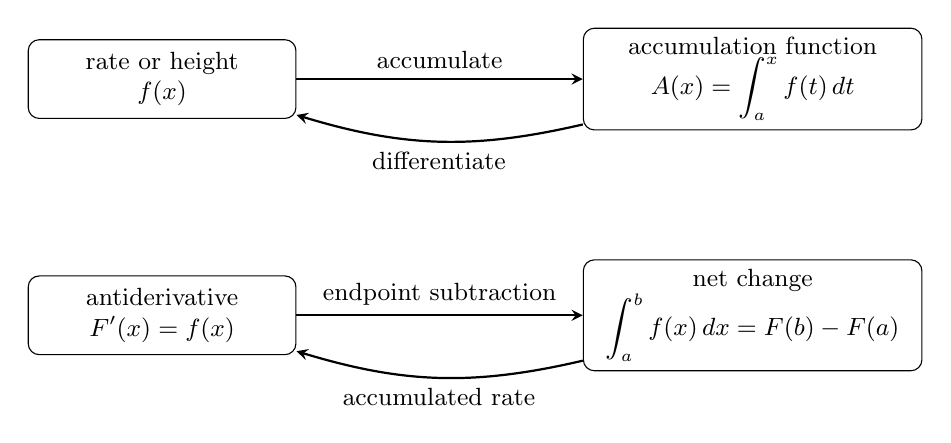
\begin{tikzpicture}[every node/.style={font=\small}, >=stealth]
  \node[draw, rounded corners, align=center, minimum width=3.4cm, minimum height=1cm] (f)
    at (0,3) {rate or height\\ \(f(x)\)};

  \node[draw, rounded corners, align=center, minimum width=4.3cm, minimum height=1cm] (A)
    at (7.5,3) {accumulation function\\ \(A(x)=\displaystyle\int_a^x f(t)\,dt\)};

  \draw[->, thick] (f) -- node[above] {accumulate} (A);
  \draw[->, thick] (A) to[bend left=15] node[below] {differentiate} (f);

  \node[draw, rounded corners, align=center, minimum width=3.4cm, minimum height=1cm] (F)
    at (0,0) {antiderivative\\ \(F'(x)=f(x)\)};

  \node[draw, rounded corners, align=center, minimum width=4.3cm, minimum height=1cm] (net)
    at (7.5,0) {net change\\ \(\displaystyle\int_a^b f(x)\,dx=F(b)-F(a)\)};

  \draw[->, thick] (F) -- node[above] {endpoint subtraction} (net);
  \draw[->, thick] (net) to[bend left=15] node[below] {accumulated rate} (F);
\end{tikzpicture}
\caption{The Fundamental Theorem connects rate, accumulation, antiderivative, and net change.}
\label{fig:chapter9-ftc-map}
\end{figure}

Here is the working summary.

\begin{center}
\begin{tabular}{p{0.20\textwidth}|p{0.45\textwidth}|p{0.25\textwidth}}
\textbf{idea} & \textbf{formula} & \textbf{meaning} \\ \hline
FTC Part I
&
\(\displaystyle \frac{d}{dx}\int_a^x f(t)\,dt=f(x)\)
&
the slope of accumulated area is the current height
\\[4mm] \hline
FTC Part II
&
\(\displaystyle \int_a^b f(x)\,dx=F(b)-F(a)\), where \(F'=f\)
&
a definite integral can be evaluated by net change
\\[4mm] \hline
net change theorem
&
\(\displaystyle \int_a^b F'(x)\,dx=F(b)-F(a)\)
&
the integral of a rate gives final minus initial
\\[4mm] \hline
indefinite integral
&
\(\displaystyle \int f(x)\,dx=F(x)+C\)
&
the family of all antiderivatives
\\[4mm] \hline
moving endpoint
&
\(\displaystyle \frac{d}{dx}\int_a^{g(x)} f(t)\,dt=f(g(x))g'(x)\)
&
FTC Part I plus the chain rule
\\[4mm] \hline
two moving endpoints
&
\(\displaystyle \frac{d}{dx}\int_{u(x)}^{v(x)} f(t)\,dt\) \newline
\(=f(v(x))v'(x)-f(u(x))u'(x)\)
&
upper endpoint adds; lower endpoint subtracts
\\[4mm] \hline
substitution
&
\(\displaystyle \int_a^b f(x)\,dx
=\int_\alpha^\beta f(g(u))g'(u)\,du\)
&
change variables using \(x=g(u)\), with \(g(\alpha)=a\), \(g(\beta)=b\)
\\[4mm] \hline
orientation
&
\(\displaystyle \int_b^a f(x)\,dx=-\int_a^b f(x)\,dx\)
&
reversing direction changes the sign
\end{tabular}
\end{center}

The most common mistakes come from forgetting one of these meanings.  A definite
integral is signed accumulation.  An indefinite integral is a family of functions.  A
substitution changes both the integrand and the limits.  A formula for an
antiderivative must be valid on the interval where it is used.

\subsection{Skills: FTC and substitution}
\label{subsec:skills-ftc-substitution}

The following problems are meant to build fluency.  In each problem, first identify
which idea is being used: FTC Part I, FTC Part II, an indefinite integral, substitution,
or orientation.

\paragraph{A. Differentiate accumulation functions.}

Assume all integrands are continuous on the relevant intervals.  Find the derivative.

\begin{enumerate}
\item

\[
G(x)=\int_1^x (t^2+1)\,dt.
\]

\item

\[
H(x)=\int_0^{x^2} e^{-t^2}\,dt.
\]

\item

\[
K(x)=\int_x^3 \sqrt{1+t^4}\,dt.
\]

\item

\[
P(x)=\int_{\cos x}^{x} (1+t^3)\,dt.
\]

\item

\[
Q(x)=\int_{x^2}^{\sin x} \frac{1}{1+t^2}\,dt.
\]

\item

\[
S(x)=\int_2^{\ln x} \sqrt{1+u^2}\,du,
\qquad x>0.
\]

\item

\[
M(x)=\int_0^x |t|\,dt.
\]

Where is \(M\) differentiable, and what is \(M'(x)\)?

\item

\[
N(x)=\int_0^{\sqrt{x}} \frac{1}{1+t^3}\,dt,
\qquad x>0.
\]

\item

\[
R(x)=\int_{1/x}^{x} \cos(t^2)\,dt,
\qquad x\neq0.
\]

\item

\[
Y(x)=\int_{\tan x}^{e^x} \sqrt{2+t^2}\,dt.
\]

\end{enumerate}

\paragraph{B. Evaluate definite integrals.}

Use antiderivatives and the Fundamental Theorem, Part II.

\begin{enumerate}
\setcounter{enumi}{10}

\item

\[
\int_0^2 (3x^2-4x+1)\,dx.
\]

\item

\[
\int_1^e \left(\frac2x+3x\right)\,dx.
\]

\item

\[
\int_0^{\pi/2}(\sin x+2\cos x)\,dx.
\]

\item

\[
\int_{-2}^2 (x^3+4x)\,dx.
\]

Explain why the answer could have been predicted from symmetry.

\item

\[
\int_{-1}^1 (x^2-x)\,dx.
\]

\item

\[
\int_0^4 \sqrt{x}\,dx.
\]

\item

\[
\int_1^8 x^{-2/3}\,dx.
\]

\item

\[
\int_0^1 \frac{1}{1+x^2}\,dx.
\]

\item

\[
\int_0^{\pi/3}\sec^2 x\,dx.
\]

\item

\[
\int_0^{\ln 2} e^x\,dx.
\]

\end{enumerate}

\paragraph{C. Indefinite integrals and initial values.}

Find the family of antiderivatives.  Then solve the initial value problems.

\begin{enumerate}
\setcounter{enumi}{20}

\item

\[
\int (5x^4-6x+7)\,dx.
\]

\item

\[
\int \left(\frac3x-4\sin x\right)\,dx.
\]

State the interval restriction.

\item

\[
\int \left(\sec^2 x+\frac{1}{1+x^2}\right)\,dx.
\]

\item Solve

\[
y'=4x^3-2x,
\qquad
y(1)=0.
\]

\item Solve

\[
s'(t)=3t^2-12t+9,
\qquad
s(0)=5.
\]

Then find

\[
s(4)-s(0).
\]

\item A population changes at the rate

\[
P'(t)=20e^{0.1t}
\]

people per year.  If

\[
P(0)=500,
\]

find \(P(t)\).

\item A temperature changes at the rate

\[
T'(t)=-6e^{-0.2t}
\]

degrees Celsius per minute.  If

\[
T(0)=80,
\]

find \(T(t)\).

\end{enumerate}

\paragraph{D. Substitution.}

Use substitution.  For definite integrals, change the limits or clearly return to the
original variable before using the original limits.

\begin{enumerate}
\setcounter{enumi}{27}

\item

\[
\int 2x\cos(x^2)\,dx.
\]

\item

\[
\int_0^2 x\sqrt{1+x^2}\,dx.
\]

\item

\[
\int_0^1 6x(1+x^2)^2\,dx.
\]

\item

\[
\int_1^e \frac{\ln x}{x}\,dx.
\]

\item

\[
\int_0^{\pi/2} \sin x\cos^3 x\,dx.
\]

\item

\[
\int_{-1}^{1}2xe^{x^2}\,dx.
\]

Explain how the substitution handles the orientation.

\item

\[
\int_0^1 \frac{2x}{1+x^2}\,dx.
\]

\item

\[
\int_0^{\pi/4}\sec^2 x(1+\tan x)^5\,dx.
\]

\item

\[
\int_0^4 \frac{1}{1+\sqrt{x}}\,dx.
\]

Use the substitution \(u=\sqrt{x}\).

\item

\[
\int_{0}^{1} \frac{x}{\sqrt{1-x^2}}\,dx.
\]

\item

\[
\int_{1}^{4} \frac{\sqrt{x}}{1+x^{3/2}}\,dx.
\]

\end{enumerate}

\paragraph{E. Mixed review.}

Choose the method.

\begin{enumerate}
\setcounter{enumi}{38}

\item Find

\[
\frac{d}{dx}\left[
x^2+\int_0^x e^{-t^2}\,dt
\right].
\]

\item Find

\[
\frac{d}{dx}\left[
\int_0^{x^3} \sqrt{1+t^2}\,dt
-
\int_0^{x} \sqrt{1+t^2}\,dt
\right].
\]

\item Evaluate

\[
\int_0^1 \left(3x^2+2x+\frac{1}{1+x^2}\right)\,dx.
\]

\item Let

\[
F(x)=\int_1^x \frac{1}{t}\,dt,
\qquad x>0.
\]

Find \(F'(x)\).  What familiar function has the same derivative and the same value at
\(x=1\)?

\item Let

\[
A(x)=\int_0^x (2+t)\,dt.
\]

Find \(A(x)\) by evaluating the integral.  Then differentiate your formula and check
FTC Part I.

\item Let

\[
B(x)=\int_x^{x^2} t^2\,dt.
\]

Find \(B'(x)\) using moving endpoints.  Then evaluate \(B(x)\) explicitly and check
your derivative.

\end{enumerate}

\subsection{Concept checks}
\label{subsec:chapter9-concept-checks}

Answer in complete sentences where appropriate.

\begin{enumerate}
\item What is the difference between

\[
\int_a^b f(x)\,dx
\]

and

\[
\int f(x)\,dx?
\]

\item In

\[
A(x)=\int_a^x f(t)\,dt,
\]

why do we usually use \(t\) instead of \(x\) inside the integral?

\item State the Fundamental Theorem of Calculus, Part I, in words.

\item State the Fundamental Theorem of Calculus, Part II, in words.

\item Why does FTC Part I require continuity at the point where we take the derivative?

\item If

\[
F'(x)=f(x),
\]

why do all antiderivatives of \(f\) on one interval have the form

\[
F(x)+C?
\]

\item Why does the constant \(C\) disappear when we use an antiderivative to evaluate
a definite integral?

\item Explain why

\[
\int_b^a f(x)\,dx=-\int_a^b f(x)\,dx.
\]

\item Give an example where

\[
\int_a^b f(x)\,dx=0
\]

but the ordinary area between the graph and the \(x\)-axis is not \(0\).

\item If \(v(t)\) is velocity, what is the difference between

\[
\int_a^b v(t)\,dt
\]

and

\[
\int_a^b |v(t)|\,dt?
\]

\item Why must the limits change when we use a substitution in a definite integral?

\item Suppose

\[
u=x^2.
\]

If \(x\) goes from \(1\) to \(3\), what are the corresponding \(u\)-limits?

\item Suppose

\[
u=1-x.
\]

If \(x\) goes from \(0\) to \(1\), what are the corresponding \(u\)-limits?  What does
this have to do with orientation?

\item Why is it dangerous to use

\[
-\frac1x
\]

as an antiderivative for \(1/x^2\) across an interval containing \(0\)?

\item Explain the sentence:

\[
\int_a^b dF=F(b)-F(a).
\]

\end{enumerate}

\subsection{Warning checks}
\label{subsec:chapter9-warning-checks}

Each item contains a tempting step.  Decide whether the step is valid.  If it is invalid,
explain exactly what went wrong.

\begin{enumerate}
\item

\[
\int_{-1}^{1}\frac1{x^2}\,dx
=
-\frac1x\Big|_{-1}^{1}
=
-2.
\]

\item

\[
\int_1^2 2x\cos(x^2)\,dx
=
\int_1^2 \cos u\,du,
\qquad u=x^2.
\]

\item

\[
\int x\,dx
=
x\int 1\,dx.
\]

\item

\[
\int_0^1 x^2\,dx
=
\int_1^0 (1-u)^2\,du,
\qquad x=1-u.
\]

\item

\[
\frac{d}{dx}\int_0^x f(t)\,dt=f(x)
\]

for every integrable function \(f\).

\item

\[
\int_{-2}^{2} |x|\,dx=0
\]

because the graph is symmetric.

\item

\[
\int \frac1x\,dx=\ln x+C
\]

on the interval \((-3,-1)\).

\item

\[
\frac{d}{dx}\int_{\sin x}^{x^2} f(t)\,dt
=
f(x^2)-f(\sin x).
\]

\item

\[
\int_0^4 \sqrt{x}\,dx
=
\int_0^2 u(2u)\,du,
\qquad x=u^2.
\]

\item

\[
\int f(x)g(x)\,dx
=
\left(\int f(x)\,dx\right)\left(\int g(x)\,dx\right).
\]

\end{enumerate}

\subsection{Proof practice: FTC Part I in a simple case}
\label{subsec:proof-practice-ftc1-simple-case}

The proof of FTC Part I rests on one idea:

\[
\frac{A(x+h)-A(x)}{h}
=
\frac1h\int_x^{x+h} f(t)\,dt,
\]

so the difference quotient is the average value of \(f\) on a short interval.  If \(f\) is
continuous at \(x\), that average must approach \(f(x)\).

The following guided proof asks you to prove this directly for

\[
f(t)=t^2
\]

without first evaluating the integral.

Let

\[
A(x)=\int_0^x t^2\,dt.
\]

Fix a real number \(x\).

\begin{enumerate}
\item Use additivity of the integral to show that

\[
A(x+h)-A(x)=\int_x^{x+h} t^2\,dt.
\]

This identity should hold for \(h>0\) and \(h<0\).

\item Show that

\[
\frac{A(x+h)-A(x)}{h}-x^2
=
\frac1h\int_x^{x+h}(t^2-x^2)\,dt.
\]

\item Suppose \(0<|h|<1\), and \(t\) lies between \(x\) and \(x+h\).  Show that

\[
|t-x|\le |h|.
\]

\item Under the same assumption, show that

\[
|t+x|\le 2|x|+1.
\]

\item Use

\[
t^2-x^2=(t-x)(t+x)
\]

to prove

\[
|t^2-x^2|\le (2|x|+1)|h|
\]

for all \(t\) between \(x\) and \(x+h\).

\item Use the order property of the integral to show

\[
\left|
\frac1h\int_x^{x+h}(t^2-x^2)\,dt
\right|
\le
(2|x|+1)|h|.
\]

\item Let \(h\to0\).  Conclude that

\[
A'(x)=x^2.
\]

\item Explain why this proof did not need an antiderivative formula for \(t^2\).

\item Repeat the same strategy for

\[
A(x)=\int_0^x (3t-1)\,dt.
\]

\item Try the same strategy for

\[
A(x)=\int_0^x t^3\,dt.
\]

What bound replaces

\[
(2|x|+1)|h|?
\]

\end{enumerate}

\begin{quote}
\textbf{What the proof tests.}
FTC Part I is not a trick for differentiating integral notation.  It is the statement that
the average height over a shrinking interval approaches the current height.
\end{quote}

\subsection{Project: reconstruct a function from its rate}
\label{subsec:project-reconstruct-function-from-rate}

A rate tells how a quantity changes.  The Fundamental Theorem tells how to rebuild
the quantity from the rate, once one starting value is known.

\[
\boxed{
Q(x)=Q(a)+\int_a^x Q'(t)\,dt.
}
\]

This project reconstructs a quantity from both an exact rate formula and sampled rate
data.

\subsubsection*{Part 1: exact reconstruction}

A tank starts with

\[
Q(0)=12
\]

liters of water.  Water flows into the tank at the rate

\[
R(t)=2+\sin\left(\frac{\pi t}{4}\right)
\]

liters per minute, for

\[
0\le t\le 8.
\]

Since \(R(t)=Q'(t)\), the amount of water in the tank at time \(x\) is

\[
Q(x)=12+\int_0^x R(t)\,dt.
\]

\begin{enumerate}
\item Write

\[
Q(x)=12+\int_0^x
\left(
2+\sin\left(\frac{\pi t}{4}\right)
\right)\,dt.
\]

\item Evaluate the integral to find an explicit formula for \(Q(x)\).

\item Find \(Q(4)\) and \(Q(8)\).

\item Differentiate your formula for \(Q(x)\).  Check that

\[
Q'(x)=R(x).
\]

\item The rate \(R(t)\) increases at first and then decreases.  Does \(Q(t)\) ever
decrease on \([0,8]\)?  Explain using the sign of \(R(t)\).

\end{enumerate}

\subsubsection*{Part 2: reconstruction from data}

Now suppose the rate is measured once per minute instead of given by a formula.

\[
\begin{array}{c|ccccccccc}
t\text{ (minutes)} & 0 & 1 & 2 & 3 & 4 & 5 & 6 & 7 & 8 \\ \hline
R(t)\text{ (liters/minute)} & 2.0 & 2.8 & 3.4 & 3.0 & 2.2 & 1.6 & 1.2 & 0.8 & 0.5
\end{array}
\]

Again assume

\[
Q(0)=12.
\]

\begin{figure}[h]
\centering
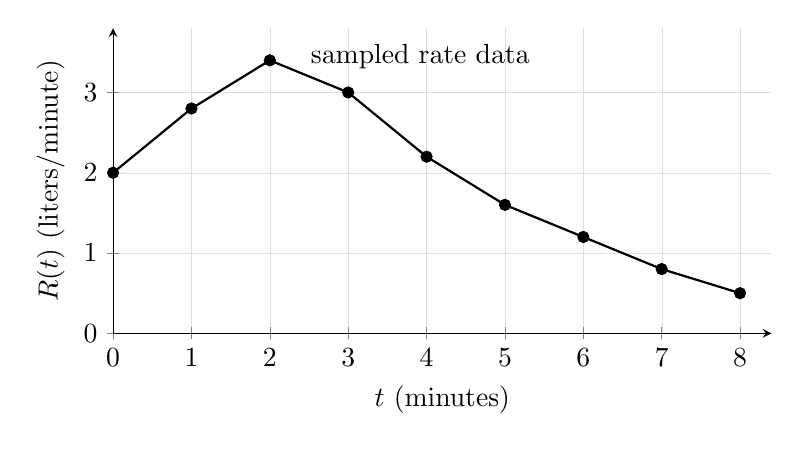
\begin{tikzpicture}
\begin{axis}[
    width=0.82\textwidth,
    height=0.45\textwidth,
    xmin=0, xmax=8.4,
    ymin=0, ymax=3.8,
    axis lines=left,
    xlabel={\(t\) (minutes)},
    ylabel={\(R(t)\) (liters/minute)},
    xtick={0,1,2,3,4,5,6,7,8},
    ytick={0,1,2,3},
    grid=both,
    grid style={line width=.1pt, draw=gray!25},
]
\addplot[only marks, mark=*] coordinates {
    (0,2.0) (1,2.8) (2,3.4) (3,3.0) (4,2.2)
    (5,1.6) (6,1.2) (7,0.8) (8,0.5)
};
\addplot[thick] coordinates {
    (0,2.0) (1,2.8) (2,3.4) (3,3.0) (4,2.2)
    (5,1.6) (6,1.2) (7,0.8) (8,0.5)
};
\node[anchor=west] at (axis cs:2.4,3.45) {sampled rate data};
\end{axis}
\end{tikzpicture}
\caption{To reconstruct \(Q(t)\), accumulate the measured rate \(R(t)\).}
\label{fig:reconstruct-from-rate-data}
\end{figure}

Use trapezoids to estimate the accumulated water.  For example, from \(t=0\) to
\(t=1\),

\[
\Delta Q
\approx
\frac12\bigl(R(0)+R(1)\bigr)(1)
=
\frac12(2.0+2.8)
=
2.4.
\]

So

\[
Q(1)\approx 12+2.4=14.4.
\]

\paragraph{Project tasks.}

\begin{enumerate}
\item Complete the cumulative trapezoid table.

\[
\begin{array}{c|c|c}
t & \text{estimated accumulated water from }0\text{ to }t & \text{estimated }Q(t) \\ \hline
0 & 0 & 12 \\
1 & 2.4 & 14.4 \\
2 & & \\
3 & & \\
4 & & \\
5 & & \\
6 & & \\
7 & & \\
8 & &
\end{array}
\]

\item Estimate the total amount of water added during the \(8\) minutes.

\item Estimate \(Q(8)\).

\item Sketch the reconstructed graph of \(Q(t)\).  It should be increasing, but its slope
should change.

\item At what time does the rate \(R(t)\) appear largest?  What does that say about the
graph of \(Q(t)\)?

\item Does the maximum of \(R(t)\) correspond to a maximum of \(Q(t)\)?  Explain.

\item Suppose the tank can hold \(30\) liters.  Based on your reconstruction, does it
overflow by \(t=8\)?

\item What additional measurements would make the reconstruction more reliable?

\end{enumerate}

\begin{quote}
\textbf{What the project tests.}
A rate graph is not the same thing as the quantity graph.  The rate tells the slope of
the quantity.  The quantity is reconstructed by accumulation.
\end{quote}

\subsection{Where this points}
\label{subsec:chapter9-hook-applications}

The Fundamental Theorem has made integration computable.

Before this chapter, a definite integral was a limit of sums:

\[
\int_a^b f(x)\,dx.
\]

Now, when we can find an antiderivative,

\[
\int_a^b f(x)\,dx=F(b)-F(a).
\]

That changes what we can do.

The next chapter asks what integrals can measure.  Area under a curve was only the
first picture.  The same accumulation idea will measure many quantities:

\[
\begin{array}{c|c|c}
\textbf{quantity} & \textbf{small piece} & \textbf{integral} \\ \hline
\text{area between curves} & \text{height difference}\cdot dx
& \displaystyle\int (\text{top}-\text{bottom})\,dx \\[8pt]
\text{volume by slices} & \text{cross-sectional area}\cdot dx
& \displaystyle\int A(x)\,dx \\[8pt]
\text{mass of a rod} & \text{density}\cdot dx
& \displaystyle\int \rho(x)\,dx \\[8pt]
\text{work by a variable force} & \text{force}\cdot dx
& \displaystyle\int F(x)\,dx \\[8pt]
\text{average value} & \text{accumulated height divided by length}
& \displaystyle \frac1{b-a}\int_a^b f(x)\,dx
\end{array}
\]

The pattern will not change:

\[
\boxed{
\text{identify a small piece, add all the pieces, and take the limit.}
}
\]

What changes is the shape of the small piece.  That is where applications of the
integral begin.
